% interactnlmsample.tex
% v1.05 - August 2017

\documentclass[]{interact}

\usepackage{epstopdf}% To incorporate .eps illustrations using PDFLaTeX, etc.
\usepackage[caption=false]{subfig}% Support for small, `sub' figures and tables
%\usepackage[nolists,tablesfirst]{endfloat}% To `separate' figures and tables from text if required
%\usepackage[doublespacing]{setspace}% To produce a `double spaced' document if required
%\setlength\parindent{24pt}% To increase paragraph indentation when line spacing is doubled
\usepackage{verbatim} 
\usepackage[capitalize,noabbrev]{cleveref}
\crefrangelabelformat{figure}{#3#1#4--#5\crefstripprefix{#1}{#2}#6}
\usepackage[numbers,sort&compress]{natbib}% Citation support using natbib.sty
\bibpunct[, ]{[}{]}{,}{n}{,}{,}% Citation support using natbib.sty
\renewcommand\bibfont{\fontsize{10}{12}\selectfont}% Bibliography support using natbib.sty
\makeatletter% @ becomes a letter
\def\NAT@def@citea{\def\@citea{\NAT@separator}}% Suppress spaces between citations using natbib.sty
\makeatother% @ becomes a symbol again

\theoremstyle{plain}% Theorem-like structures provided by amsthm.sty
\newtheorem{theorem}{Theorem}[section]
\newtheorem{lemma}[theorem]{Lemma}
\newtheorem{corollary}[theorem]{Corollary}
\newtheorem{proposition}[theorem]{Proposition}

\theoremstyle{definition}
\newtheorem{definition}[theorem]{Definition}
\newtheorem{example}[theorem]{Example}

\theoremstyle{remark}
\newtheorem{remark}{Remark}
\newtheorem{notation}{Notation}
\usepackage[utf8]{inputenc} % usually not needed (loaded by default)
\usepackage[T1]{fontenc}
\usepackage{tikz}
\usepackage{enumerate}
\usepackage[section]{placeins}
\usetikzlibrary{positioning}
\usepackage{caption}
\usepackage{array}
\usepackage{amsmath}
\graphicspath{D:\paper1 (2)\Paper Work\Paper Measuring wheelset}

\begin{document}

\articletype{RESEARCH ARTICLE}% Specify the article type or omit as appropriate

\title{Measuring Wheel-Set Design}

\author{
\name{Chetan Zambare\textsuperscript{a} and N. S. Vyas\textsuperscript{b}} \thanks{CONTACT: Nalinaksh S. Vyas. Email: vyas@iitk.ac.in. Department of Mechanical Engineering, Indian Institute of Technology Kanpur, Kanpur 208016, Uttar Pradesh, India.}
\affil{Department of Mechanical Engineering, Indian Institute of Technology Kanpur, Kanpur, Uttar Pradesh -208016, India}
}

\maketitle

\begin{abstract}
Rail-wheel contact forces significantly affect dynamic behaviour and derailment of a train. The aim is to develop a unique method that provides continuous measurement of rail-wheel contact forces and contact point position using a measuring wheel-set. Numerical simulation of vehicle behaviour is performed in SIMAPCK and use these results as an input parameter for performing FEM calculations. The study addresses critical issues in development measuring wheel-Set, such as to locate strain sensitive radial location in the wheel, determining optimal location, number, and way of connecting strain gauges. The relation between strain in the wheel and the input parameter is formulated and verified using the FEM study. The percentage error involved in calculating the contact force is less than 1 \%, and the percentage error involved in predicting the contact point position is less than 4 \%. 
\end{abstract}

\begin{keywords}
Instrumented Wheel-Set, Finite Element Analysis, Multibody Simulation 
\end{keywords}


\section{Introduction}
The railways in India are the principal mode of transportation for freight and passengers. It is a vital task of Indian railways to run these vehicles under the highest safety in all standard and emergency manoeuvres. The rail-wheel contact force plays a prominent role in rail-road vehicle dynamics. It is an essential measure for a proper understanding of railway vehicle dynamic  behaviour and derailment risk.  The rail and wheel profile is non-linear. The calculation of these contact forces for two interacting non-linear bodies is essential, as they cause a lot of unwanted effects such as vibration, wear, fatigue, noise, thermal effect. Accurate measurement of these forces is one of the critical problems in railway vehicle dynamics. Many researchers had worked on calculating the contact forces. De Peter A \cite{Pater1,Pater2} has studied the geometrical contact between the rail and wheel. Constraint equations are generated at rail-wheel contact. Hertz \cite{Hertz} has studied contact between two spheres having a non-linear profile at contact. The contact patch would be elliptical, and pressure distribution over the contact patch will be semi-elliptical. The size of this contact ellipse is the function of transverse radii of wheel and rail, rolling radius of the wheel, axle load, and material of wheel and rail. Carter \cite{Carter} introduced the fundamental concept of creep forces and gave a solution, for the two-dimensional case of two long cylinders pressed together by a normal force and transmitting a tangential force across the contact stripe. Kalkar \cite{Kalker1,Kalker2,Kalker3,Kalker4} studied the rail wheel contact as a three-dimensional case and gave linear creep theory for computing the creep forces. He also tabulated the creep coefficient as a function of the size of the contact ellipse. He has also given the FASTSIM algorithm \cite{Kalker5}, which is used in many Multi-body software software to calculate rail-wheel contact forces.

There are two measuring approaches way-side (track-side) approach and vehicle side approach. Way-side  measurement technique is a discrete force measurement technique. In this technique, different locations are selected on a rail to place the sensors, which helps to calculate the contact forces when the train passes on that location. Akira Mastuomoto \cite{Matsumoto} has worked on the way-side system. The Independent Component Analysis (ICA) with system calibration is used to successfully separate vertical Force and lateral Force from recorded strain signal. ORE \cite{ORE} measured contact forces by measuring rail distortion with strain gauges.  The second approach is the measurement from the vehicle side. Some researchers are working on-board measuring technique. Placing sensors on the axle box and predicting forces from that that signal. Fi Xia \cite{Fxia,Fxia1} developed an inverse railway wagon model and predicted contact forces using acceleration data.   Kalman filter approach \cite{Chris,Ward,Lic} has been used to predict creep forces that are used to predict contact forces.                      

The wheel is directly affected due to contact force variation; hence the instrumented wheel-set is the most accurate method for the measurement of contact forces. In this approach wheel act as a sensor for contact force and contact point variation. Based on the signal obtained from the Wheatstone bridge, contact forces can be predicted. Yu Ren \cite{Yu}  measured rail-wheel contact forces using state-space theory. During normal running of the vehicle as sampling frequency is high compared to the frequency of forces, the current state of forces is dependent on the previous state of forces. The recurrence relationship between strain in wheel and forces is formulated. The different bridging scheme gives different trigonometric series with a different active harmonic component. A strong tracking Kalman filter and particle filter were effective methods while calculating contact forces from a signal from Wheatstone bridge. Milan B Baize \cite{Milan}  has worked on an instrumented wheel-set. He has addressed critical issues like wheel disk sensitivity under the effect of variation of contact forces, the optimal way of connecting these strain gauges. He has used the inverse identification method. For measurement of an n input signal, the n output signal is measured, and the recorded mixture of output signal will be linear combinations of the original signal. Xincan Jin \cite{Xincan}  has worked on wheel-set roller rig; load time history is applied on a wheel that generated running conditions. Calibration is done by using the minimization approach to formulate transfer function between strain and contact forces. Bagheri \cite{Bagheri}  Strain measured from strain gauge is dependent on wheel rotation. He has worked on placement of strain gauges in on measuring wheel. Fourier series expansion is performed on strain signal, it has observed that amplitude of first harmonic is greater than other harmonics. Placement of strain gauge in Wheatstone bridge is done in such a way that higher harmonics cancels each other.
      
  There are significantly fewer publications that have addressed the critical problems that occurred during the measuring wheel development. Detail derivation of the mathematical relationship between a strain with rail-wheel contact forces and the contact point variation is given in the following study. Much of the research work in measuring wheel-set focuses on acquiring a Wheatstone bridge signal and deriving contact forces and contact point locations from the strain signal's calibration. Detail procedure behind FEM analysis of wheel and critical issue in FEM analysis is discussed in the following study. Numerical simulation is performed in SIMPACK to get important information about the contact patch and contact point variation under practical constraints. This information is used in the FEM study to explicitly address the critical issue of locating radial location by finding out strain sensitive location in the wheel under the effect of variation of contact forces and the contact point, determining optimal location number, and connecting strain gauges in Wheatstone bridge. 

\subsection{Problem formulation}
The objective of the study is to measure contact forces and contact point location from strain measured from strain gauges which are placed on the wheel. Strain in the wheel is affected by lateral force (Q), vertical force (F), longitudinal force (X), contact point (L), moment (M), angular velocity ($\omega$), wear (w) and temperature (T) as given by \cref{eq:strain}.
\begin{equation}
Strain(\epsilon) = \emph{f}(Q,F,X,L,\omega,M,w,T) \label{eq:strain}
\end{equation}
In the following study, the effect of wear and temperature is neglected. Longitudinal force (X) acts in the direction of vehicle movement. Kalkar coefficient, which is needed to calculate moment, is small; hence moment term can be neglected. The main task of stress-strain analysis is the identification of wheel sensitivity for individual application of lateral force, vertical force as well as a change in the contact point position. It is important to find the optimum layout, number, and way of connecting strain gauges to obtain continuous signals and reliable reading. The mathematical relation between the output signal and the input signal needs to be formulated after placing strain gauges at these locations.
Problem is classified into two segments is shown in \cref{fig:formulation}.
\begin{itemize}
\item Forward problem
\item Inverse problem
\end{itemize}


\begin{figure}
\centering
\resizebox*{11cm}{!}{\includegraphics{formulation.jpg}}
\caption{Problem Formulation} \label{fig:formulation}
\end{figure}


\section{The Mathematical Formulation of the Relationship between Strain in a Wheel and Contact Forces}
\subsection{Kinematic oscillations of wheel-set}
Rail-wheel contact is special contact. When small irregularity comes, wheel-set laterally displaces from its mean position, and both wheels will be exposed to different diameters, as shown in \cref{fig:differentradius} . Due to this, both wheels will have different peripheral velocity. A higher diameter wheel will have higher velocity, and others will lose the ground but will regain on its progress. The process of alternatively gaining and losing ground of each other will cause the wheel to proceed in oscillatory motion, as shown in the \cref{fig:kinematicoscillation}. Due to this oscillation wheel-set move in snake-like motion on the rail. The frequency of oscillation is called kinematic oscillation [19]. Due to these contact patch varies in a lateral direction as the vehicle moves forward.


\begin{figure}
\centering

\subfloat[][Wheel-set displaced in lateral direction]{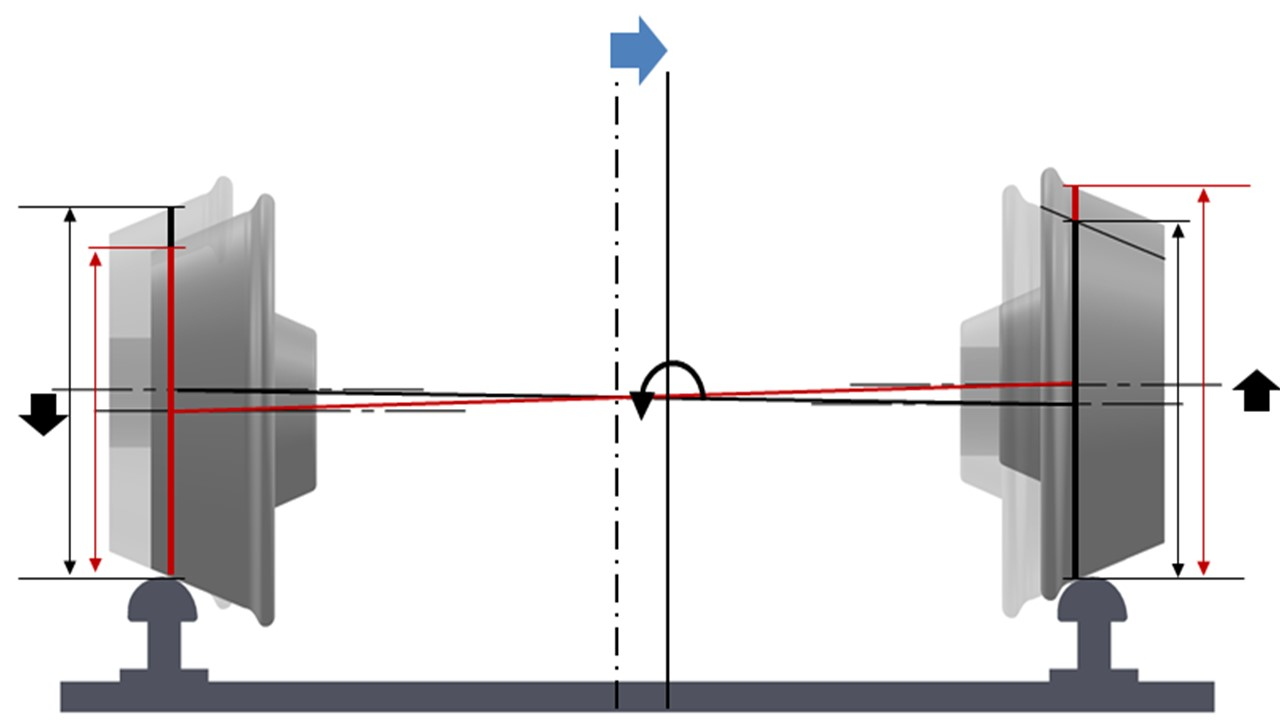
\includegraphics[scale=0.2]{2.1.aWheeldisplacement.jpg}
\label{fig:differentradius}}
\subfloat[][wheel-set movement]{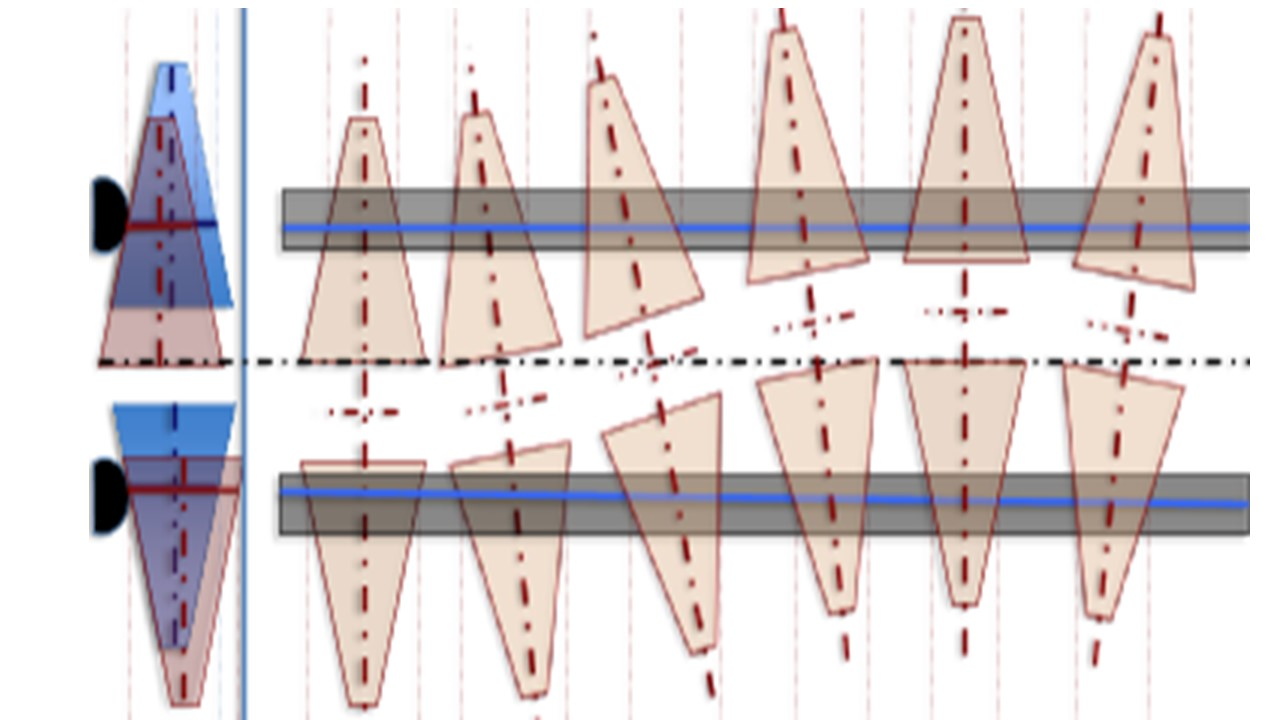
\includegraphics[scale=0.2]{2.1.bKlnigelfrequency.jpg}\label{fig:vehiclemovement}}
\caption{Kinematic oscillation of wheel-set}
\label{fig:kinematicoscillation}
\end{figure}

\subsection{Contact forces}
When two elastic bodies wheel and rail pressed against each other to transfer normal load, a contact patch is generated at rail-wheel interaction. The contact forces at rail-wheel interaction are a function of creep and creep coefficient calculated by Kalakar’s theory [5]. The Figure  \ref{fig:FBD} shows force acting at rail-wheel interaction. Due to the kinematic oscillation of a wheel-set in a lateral direction, the slope at a contact point also varies. Hence contact forces vary as the vehicle moves forward.

\begin{figure}[h]
\centering
\subfloat[Force acting on rail ]{%
\resizebox*{7cm}{!}{\includegraphics[scale=0.6]{contactforces1.jpg}}}\label{fig:forceonrail}
\subfloat[ Force acting on left wheel ]{%
\resizebox*{7cm}{!}{\includegraphics[scale=0.1]{crosssection1.jpg}}}\label{fig:crosssection}
\caption{Free body diagram at rail-wheel interaction} \label{fig:FBD}
\end{figure}

\subsection{Determination of strain at measuring point under the effect of contact forces.}
\begin{figure}[h]
\centering
\resizebox*{10cm}{!}{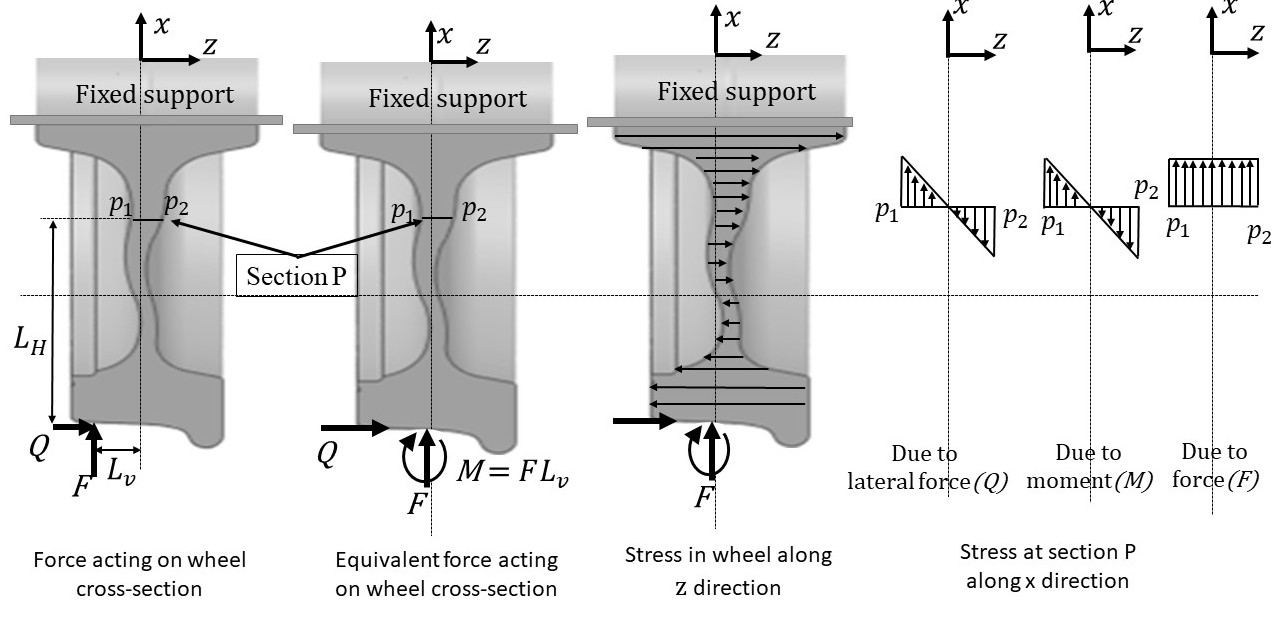
\includegraphics[scale=0.6]{Stressesinwheel.jpg}}
\caption{Stress in wheel cross-section due to contact forces} \label{fig:stress}
\end{figure}

\subsubsection{Stress at measuring point due to vertical force}

The distance $L_V$ of the vertical force from the neutral axis is   shown in \cref{fig:stress}. The effect of vertical force on section P in wheel is similar to axial force passing through the neutral axis and equivalent moment measured from the neutral axis.  stress at $x$ direction produced at the measuring point is  given by \cref{eq2}. z is the distance of measuring point from the neutral axis, and I is the moment of inertia of the wheel.
\begin{equation}
\sigma_p= \sigma_{bending}+ \sigma_{direct} \label{eq1}
\end{equation}
\begin{equation}
\sigma_p= \frac{FL_Vz}{I} +   \frac{F}{A_{normal}}   \label{eq2}
\end{equation}


\subsubsection{Stress at measuring point due to lateral force}

The wheel behaves as a cantilever beam under the action of lateral force. The section near to fixed support is stress sensitive. Lateral force produces bending stress in section P, as shown in \cref{fig:stress}. The distance of the lateral force from the measuring point is $L_H$. Bending stress produced due to lateral force is given by \cref{eq3}. If lateral force is displaced in a lateral direction, variation in  $L_H$ is negligible as the measuring point is fixed. Hence there is significantly less variation in stress at the measuring point due to lateral force variation in a lateral direction.  

\begin{equation}
\sigma_p= \frac{QL_Hz}{I}    \label{eq3}
\end{equation}

Stress in the wheel is a function of both contact forces. The measuring point is fixed. The stress-strain relationship can be formulated by Hooke’s law, which dependent on the material. After taking out constant term strain at a measuring point $P_1$ is given by \cref{eq4}.
\begin{equation}
\epsilon_p=  \theta_{P1}F+ \theta_{P2}FL_V+ \theta_{P3}Q     \label{eq4}
\end{equation}

\section{Numerical Simulation of Vehicle Behaviour}
It is essential to know about contact point variation and contact patch dimension for a running vehicle as they affect contact force acting on a wheel. Numerical simulation is performed in SIMPACK on an equivalent wheel-set model that replaces the actual system under practical constraints. Wheel profile IRS R-19/93 and rail profile UIC 60 is used to generate wheel-set in SIMPACK, as shown in \cref{fig:Wheelset}. Special Hertzian contact is used at rail wheel interaction. FASTSIM algorithm formulated by Kalkar is used to measure rail-wheel contact forces. Simulation is performed for v =10 m/s, and the result is plotted for the right wheel.  The lateral displacement of the wheel-set from a mean position is shown in the \cref{fig:lateraldisp}. The dimension of a contact patch variation with lateral displacement is shown in the \cref{fig:Contactpatch}. \cref{fig:length} shows that contact patch length is almost constant, having a dimension of 6.4 mm, and it is minimum when the flange touches the rail. \cref{fig:width} shows that contact patch width is almost constant, having a dimension of 1 mm, and it increases when flange touches the rail. The equivalent dimension of faces is generated on the CAD model of the wheel face. The Wheel-set displaces from the mean position is from  -2.5 mm to +2.5 mm.
\begin{figure}
\centering
\resizebox*{8cm}{!}{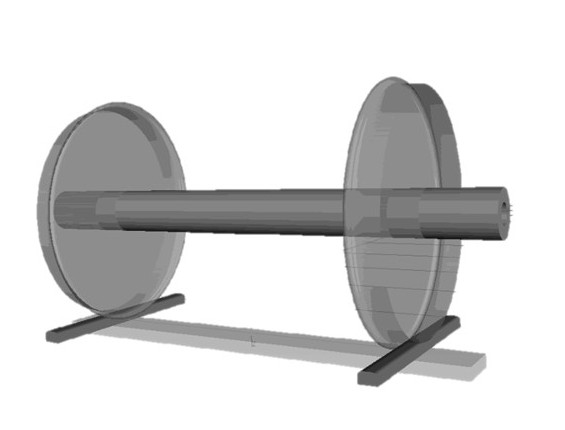
\includegraphics{Wheelset.jpg}}
\caption{Equivalent wheel-set model generated in SIMPACK} \label{fig:Wheelset}
\end{figure}
\begin{figure}
\centering
\resizebox*{8cm}{!}{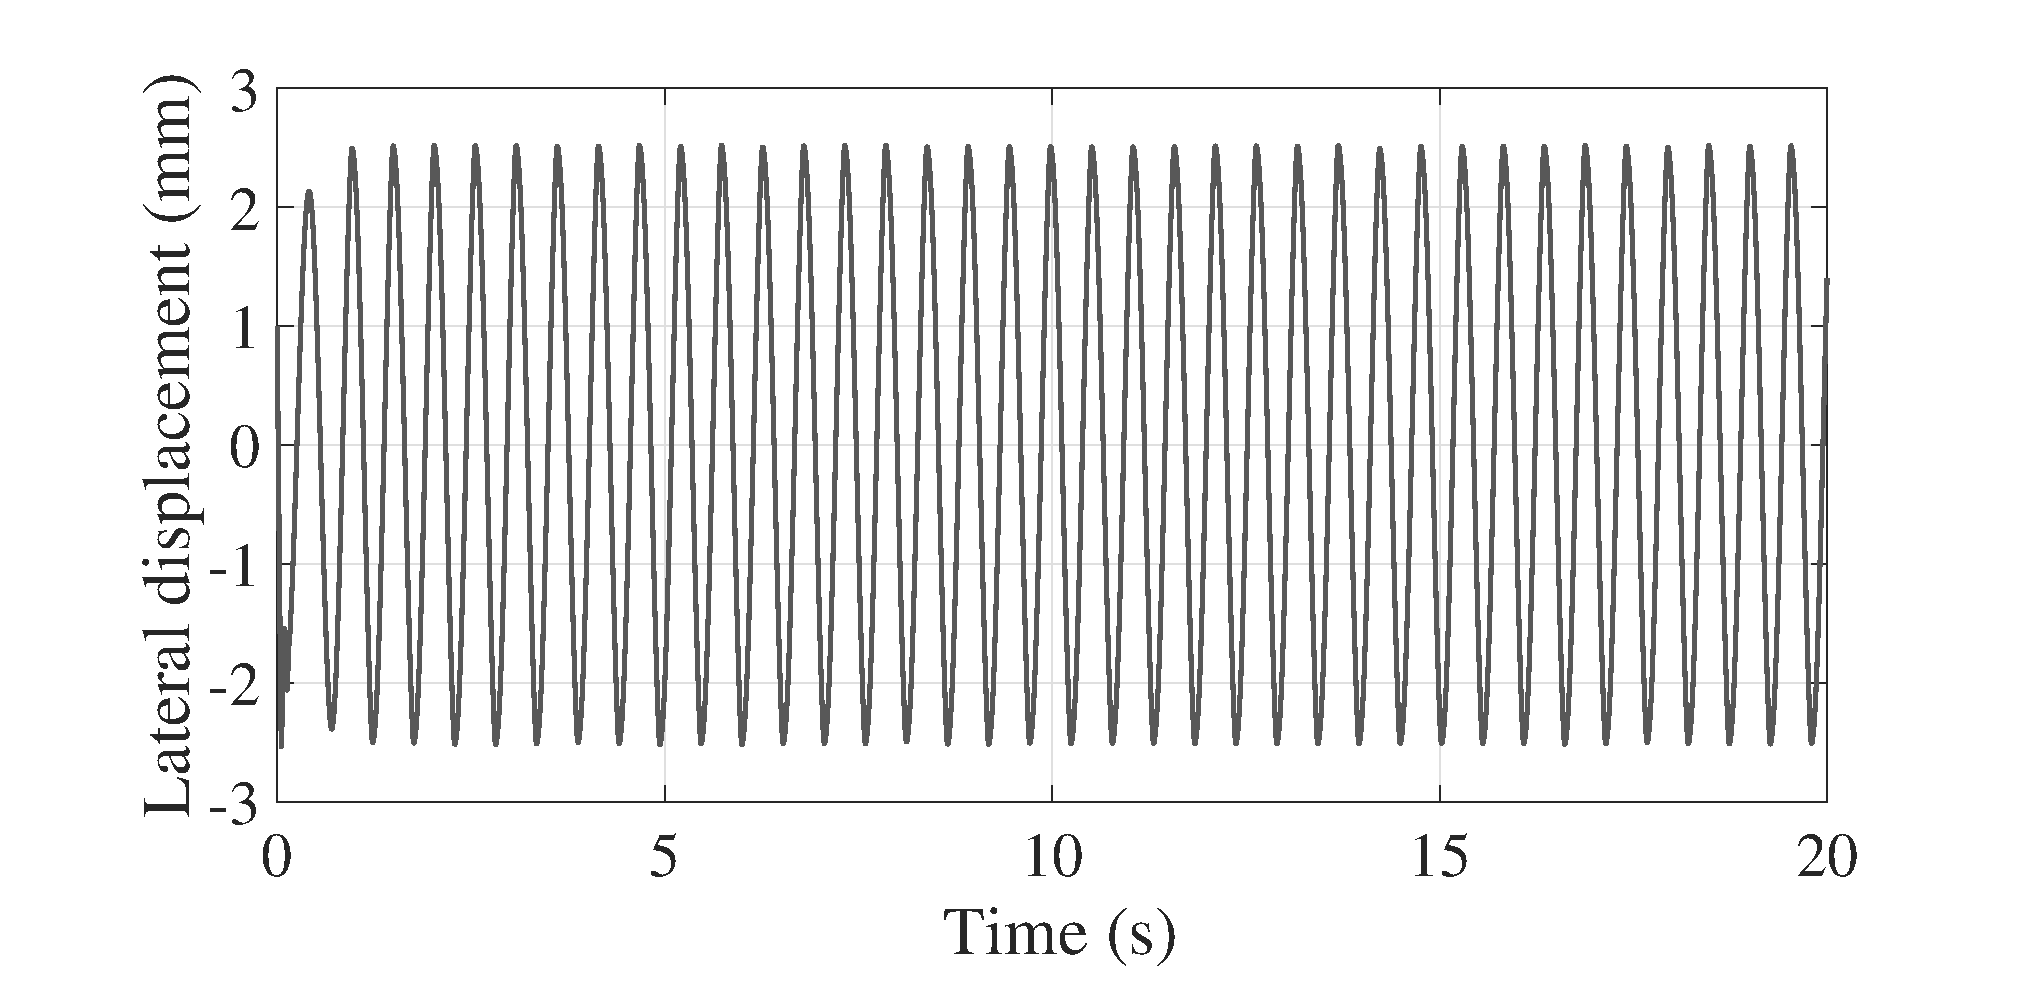
\includegraphics{lateraldisp.eps}}
\caption{Lateral displacement of wheel-set } \label{fig:lateraldisp}
\end{figure}
\begin{figure}
\centering
\subfloat[][Length of contact patch  ]{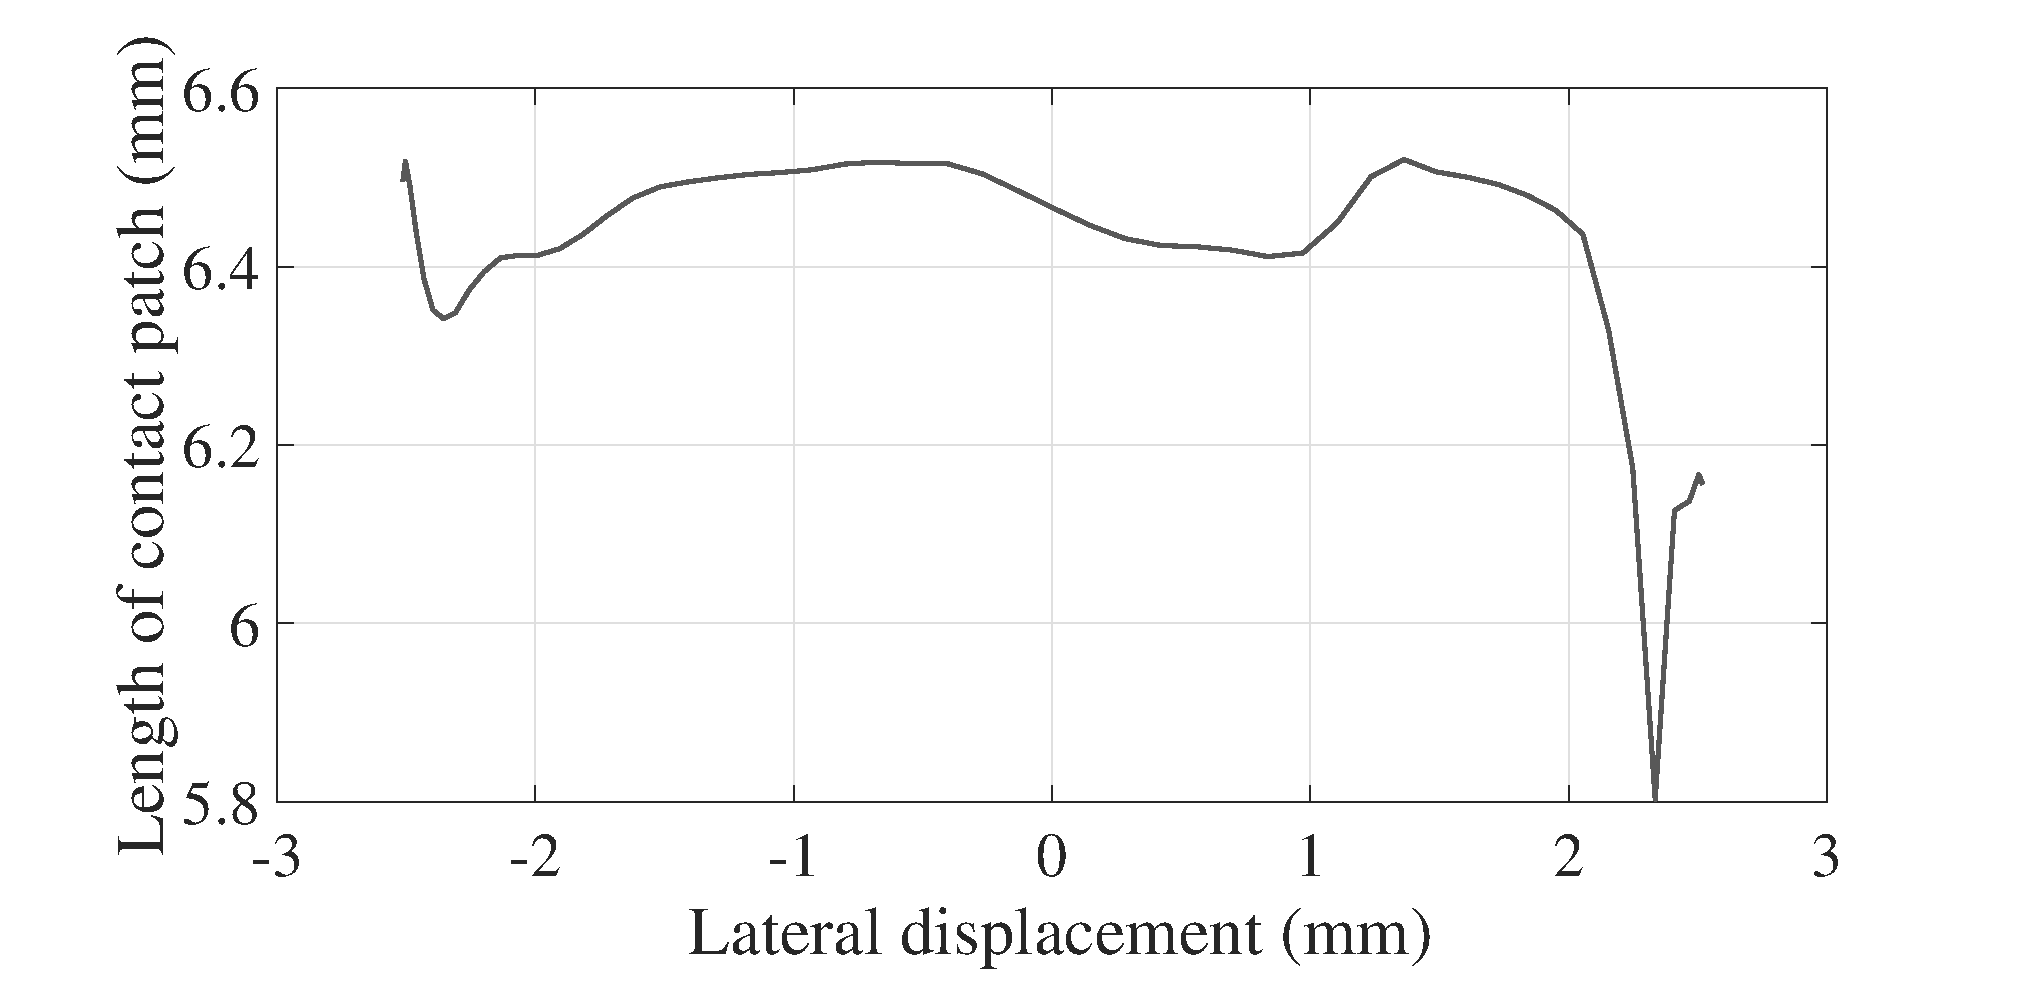
\includegraphics[scale=0.2]{contact_length.eps}
\label{fig:length}}
\subfloat[][Width of contact patch ]{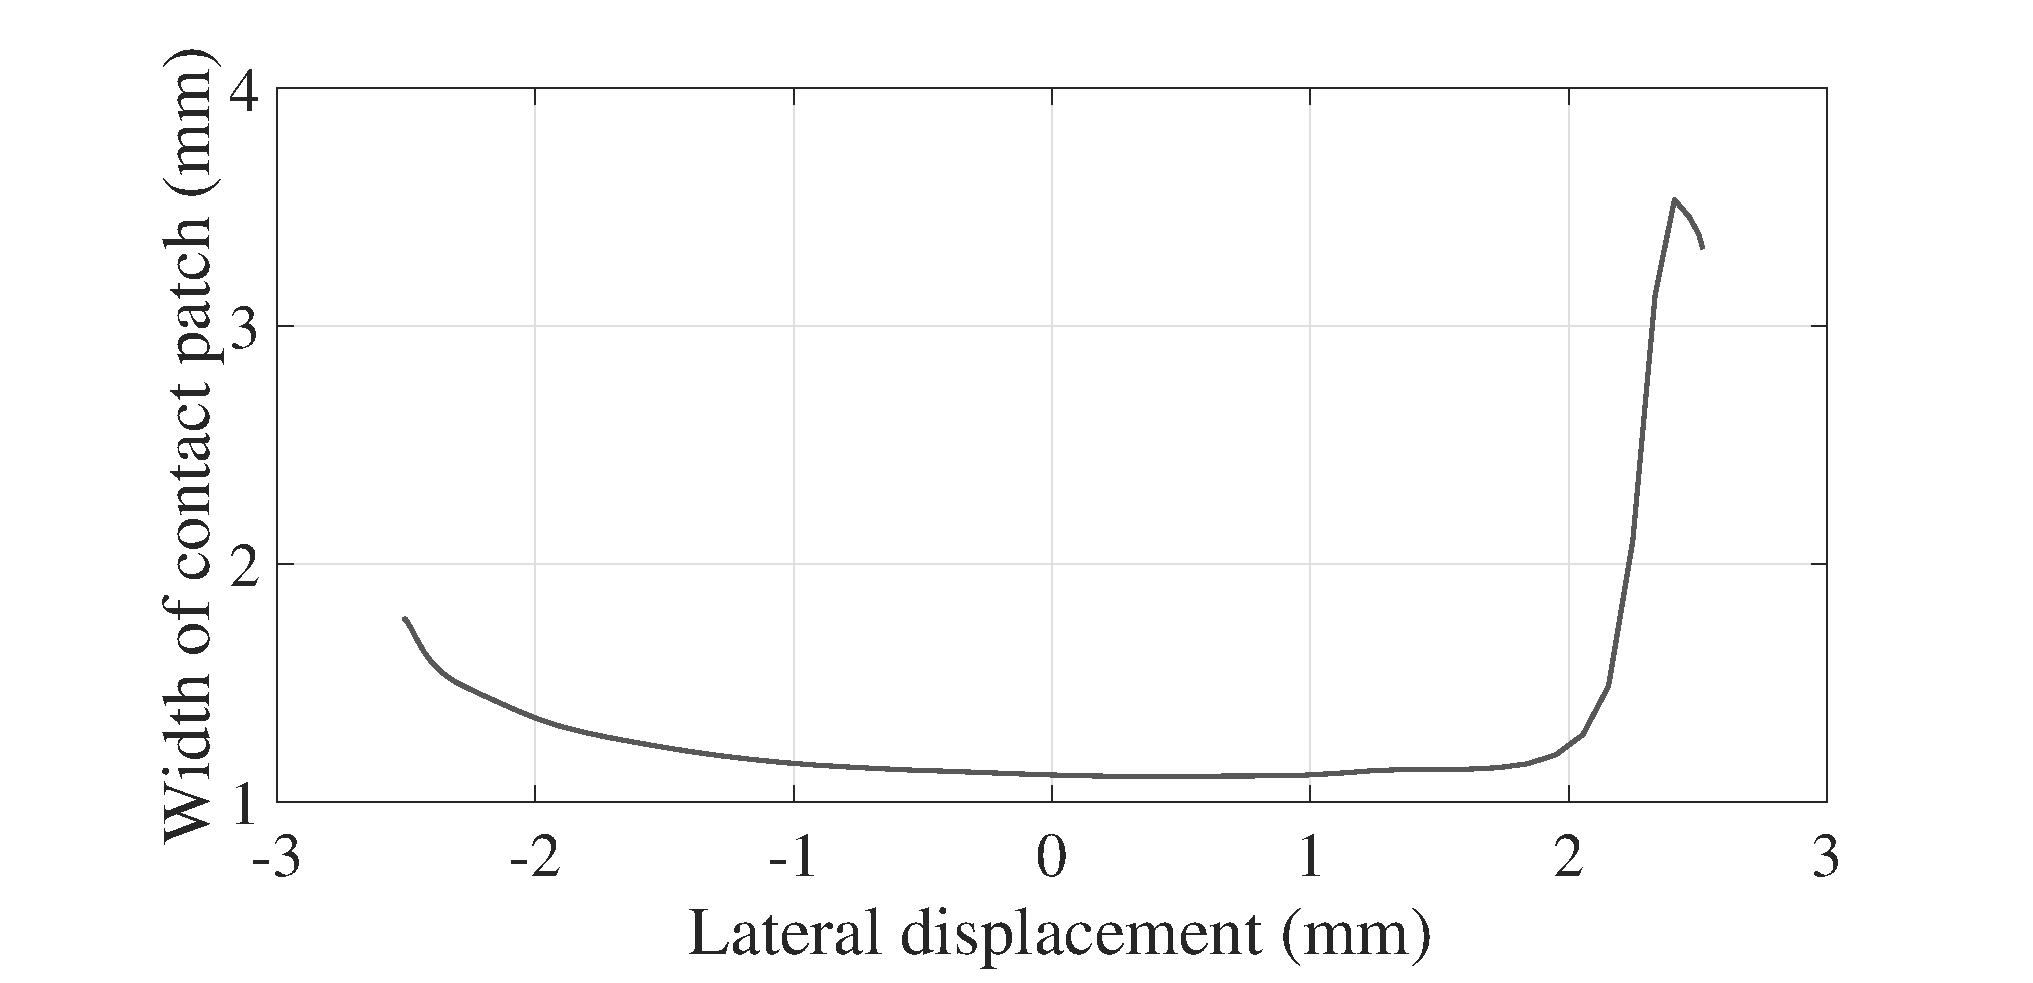
\includegraphics[scale=0.2]{contactwidth.eps}\label{fig:width}}
\caption{Contact patch variation with lateral displacement of wheel-set}
\label{fig:Contactpatch}
\end{figure}

\section{Finite Element Analysis of Wheel.}


The wheel model (IRS R19-93) is used in the following study. Finite element analysis is performed in ANSYS workbench FE package. \cref{fig:Meshwheel} shows the meshed model of the wheel. Material properties are shown in Table \ref{tab1}. The finite element model properties are shown in Table \ref{tab2}.
\begin{figure}[h]
\centering
\resizebox*{6cm}{!}{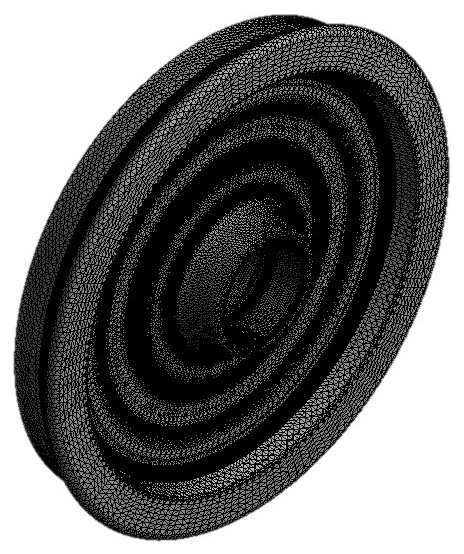
\includegraphics{Meshwheel.jpg}}
\caption{Finite element model of wheel} \label{fig:Meshwheel}
\end{figure}

\begin{table}[h]
\tbl{Material properties for wheel}
{\begin{tabular}{ll}
\toprule
Properties & Value\\
 \midrule
 Densisty & 7850  \\ 
 Modulus of Elasticity & 200 Gpa  \\ 
 Bulk modulus & 166.67 Gpa  \\ 
 Shear modulus & 76.92 Gpa  \\ 
Poisson ratio &	0.3  \\

\bottomrule
\end{tabular}}
\label{tab1}
\end{table}

\begin{table}[h]
\tbl{Finite element model properties for wheel}
{\begin{tabular}{lll}
\toprule
 Type of element & No. of nodes & No of elements  \\ 
 \midrule
SOLID187 &	431450 &	726327  \\
 
\bottomrule
\end{tabular}}
\label{tab2}
\end{table}

The wheel is displaced in a lateral direction in a range of +3 mm and -3 mm from the mean position of the wheel-set as shown in fig. Rail-wheel interaction generates an elliptical patch. A rectangular patch is created on the wheel of an equivalent area instead of an elliptical patch.  In the angular direction, the wheel face is divided into 160 faces. In the lateral direction, the wheel is divided into 24 faces with a dimension of 0.5 mm each. The rectangular patch near the flange side is numbered as contact patch 1

.  The rotational velocity effect is given to the wheel to consider the effect of centrifugal acceleration at a measuring point on the wheel. 

The main task of FEM study is the identification of wheel sensitivity for individual application of lateral force, vertical force, and change in the contact point position. The optimum choice of strain sensitive radial distance for placing the strain gauges allows us to calculate contact forces. Proper angular position selection for placing the strain gauges and connecting them in Wheatstone bridge reduces dependency between the Wheatstone bridge signal and angular velocity. 
The complete analysis can be broken down into the following steps.
\begin{itemize}
\item Determination of strain sensitive radial location on the wheel
\item  Optimum number and way of connecting strain gauge in Wheatstone bridge
\end{itemize}
\subsection{Determination of strain sensitive radial location on the wheel.}
It is crucial to identify the strain sensitive radial location by analysing the effect of lateral force, vertical force, and contact patch on strain in the wheel. There are two choices for strain gauge placement one for the wheel’s inner side and the other on the wheel’s outer side. The path is created on the wheel in the inner and outer direction that varies radially. The most strain sensitive location in the wheel under the effect of vertical force and lateral force is explored by analysing the following case.
\begin{itemize}
\item Effect of vertical force variation on strain in radial direction on the wheel
\item  Effect of lateral force variation on strain in radial direction on the wheel
\end{itemize}

\subsubsection{Effect of vertical force variation on strain in radial direction on the wheel}
The constant vertical load of 100 KN is applied on the wheel at a contact patch that varies only in a Lateral direction as shown in                     \cref{fig:verticalforcevariation}. From a \cref{fig:strainvertical}, the inner side r = 155.9 mm and at the outer side r = 214.3 mm locations are strain sensitive under vertical force. The strain is always maximum at these locations, even if vertical force varied in the lateral direction.
\begin{figure}[h]
\centering
\resizebox*{10cm}{!}{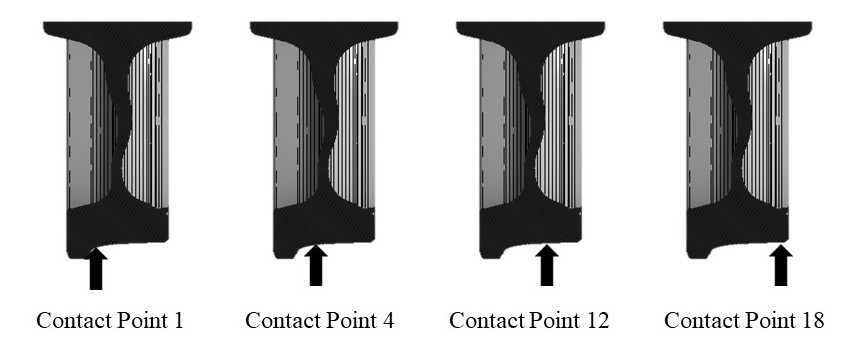
\includegraphics[width=1.5\linewidth,height=0.5\textheight]{verticalforcevariation.jpg}}
\caption{ Vertical force variation} \label{fig:verticalforcevariation}
\end{figure}

\begin{figure}
\centering
\subfloat[Strain at inner side of wheel]{%
\resizebox*{7cm}{!}{\includegraphics[width=1.0\linewidth,height=0.35\textheight]{verinner.eps}}}
\subfloat[Strain at outer side of wheel]{%
\resizebox*{7cm}{!}{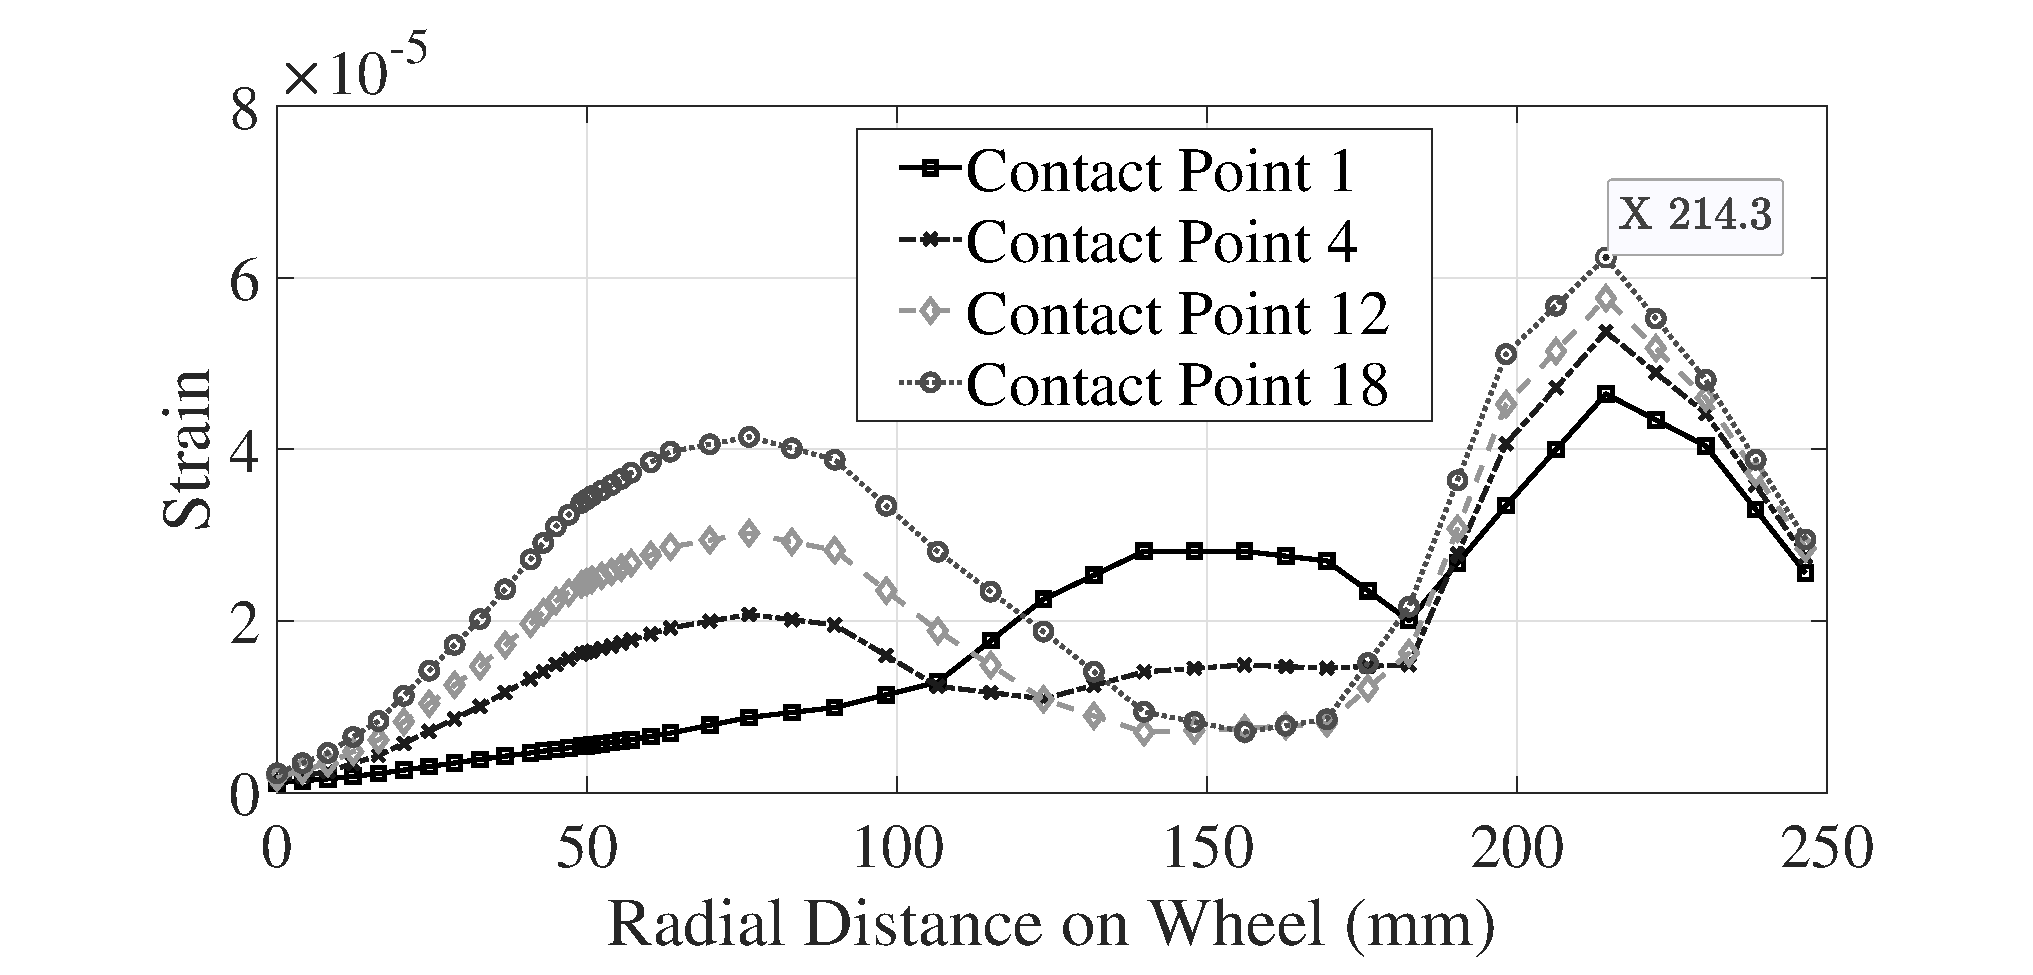
\includegraphics[width=1.0\linewidth,height=0.35\textheight]{verouter4.eps}}}
\caption{Strain sensitive radial location due to vertical force } \label{fig:strainvertical}
\end{figure}


\subsubsection{Effect of lateral force variation on strain in radial direction on the wheel}
The constant vertical load of 20 KN is applied on the wheel at a contact patch that varies only in a Lateral direction as shown in   \cref{fig:horizontalforcevariation}. From a \cref{fig:strainvertical}, the inner side r = 63.14 mm and at the outer side r = 55.13 mm locations are strain sensitive under vertical force. The strain is always maximum at these locations and it is independent of lateral force variation in lateral direction. 

Radial location A, B, C, as shown in the \cref{fig:Radiallocation}  is chosen for placing the strain gauges on the wheel. Location C is sensitive to lateral force variation as it is far away from the point of application of force. Point A, B are sensitive to vertical force variation because the normal area is less in these sections.

\begin{figure}[h]
\centering
\resizebox*{10cm}{!}{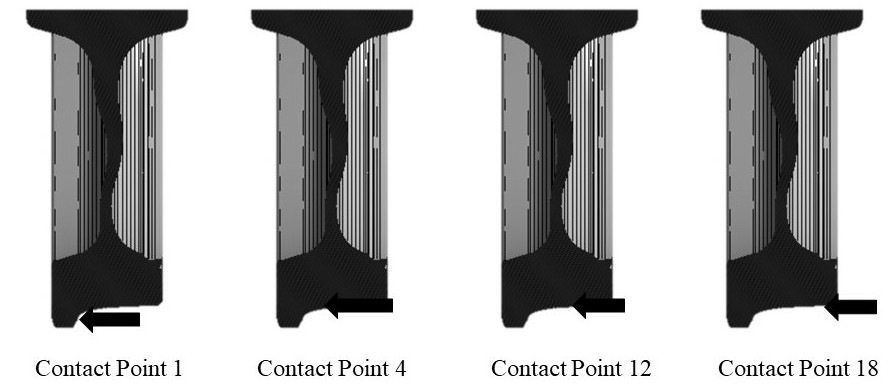
\includegraphics[width=1.5\linewidth,height=0.5\textheight]{horizontalforcevariation.jpg}}
\caption{ Lateral force variation} \label{fig:horizontalforcevariation}
\end{figure}


\begin{figure}[h]
\centering
\subfloat[Strain at inner side of wheel]{%
\resizebox*{7cm}{!}{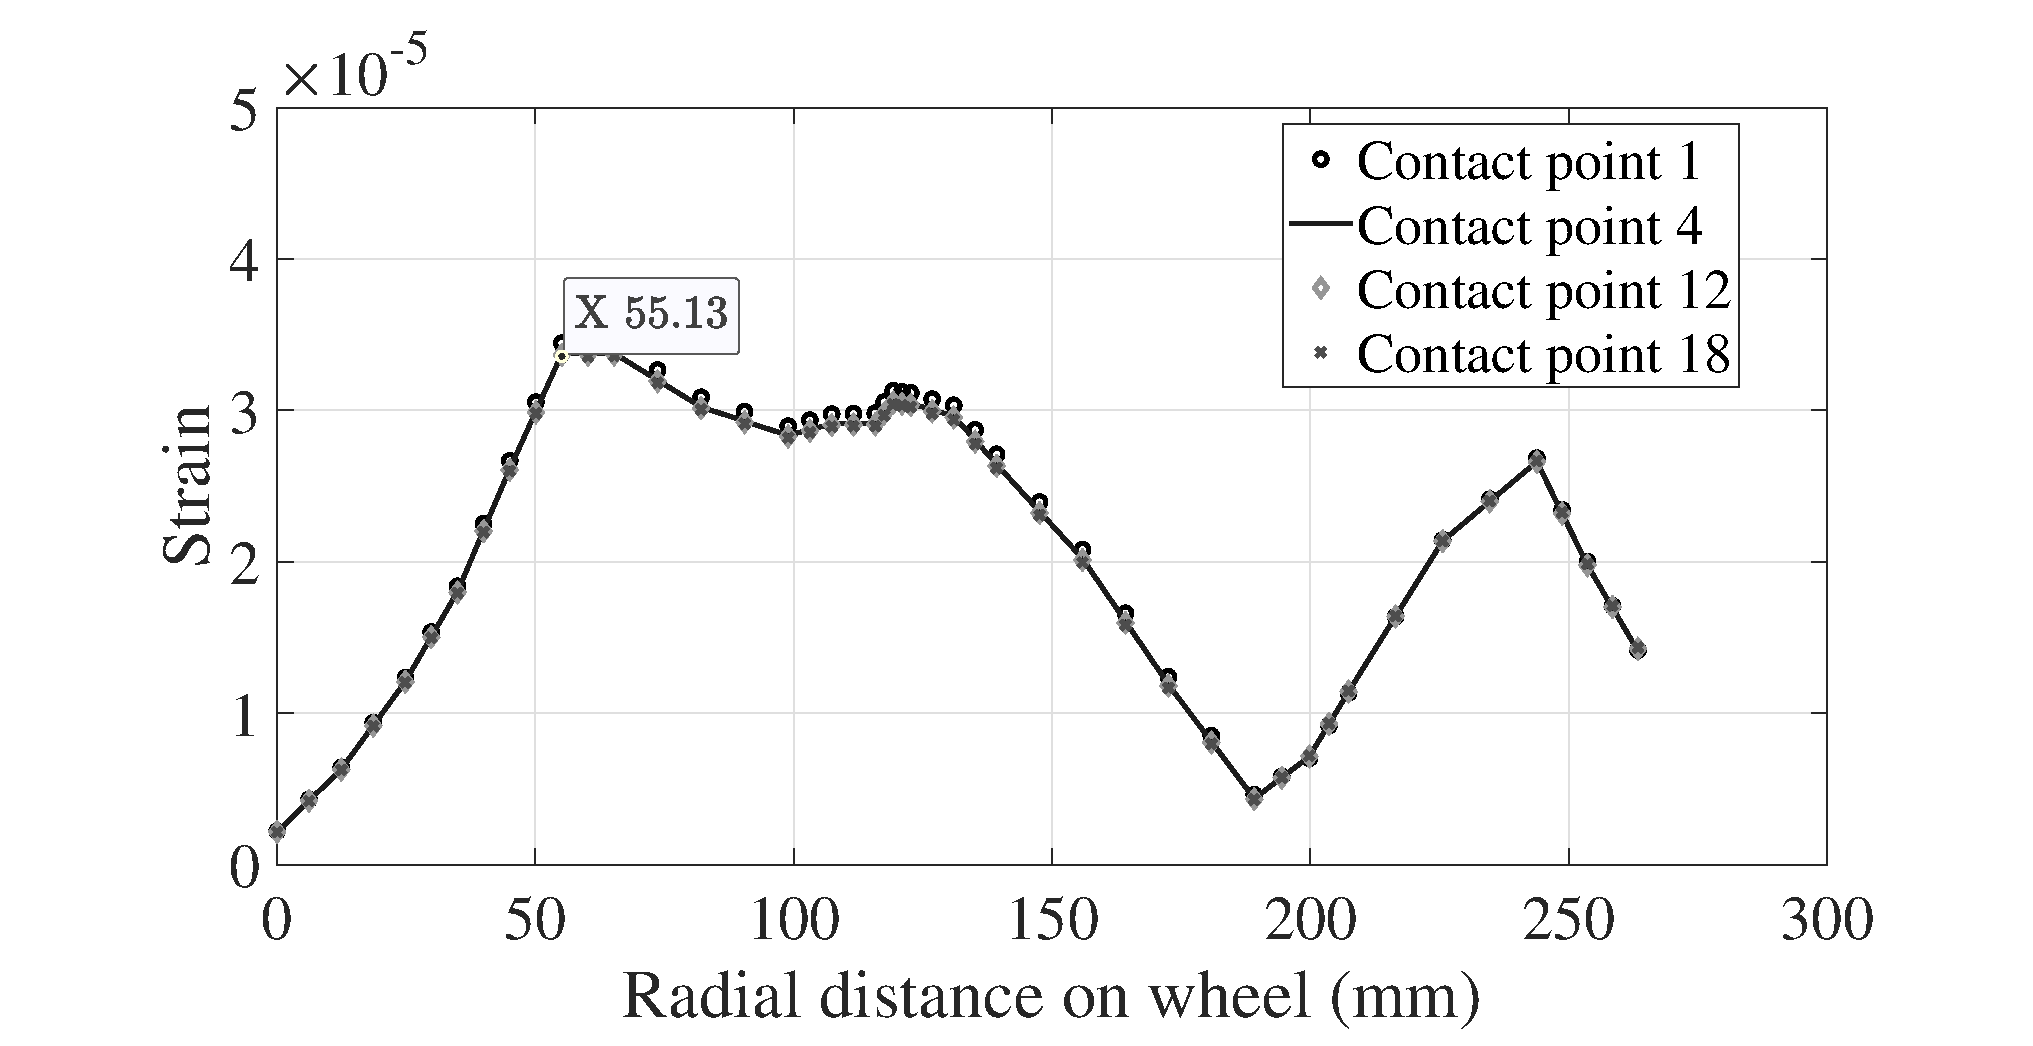
\includegraphics[width=1.0\linewidth,height=0.35\textheight]{latinn.eps}}}
\subfloat[Strain at outer side of wheel]{%
\resizebox*{7cm}{!}{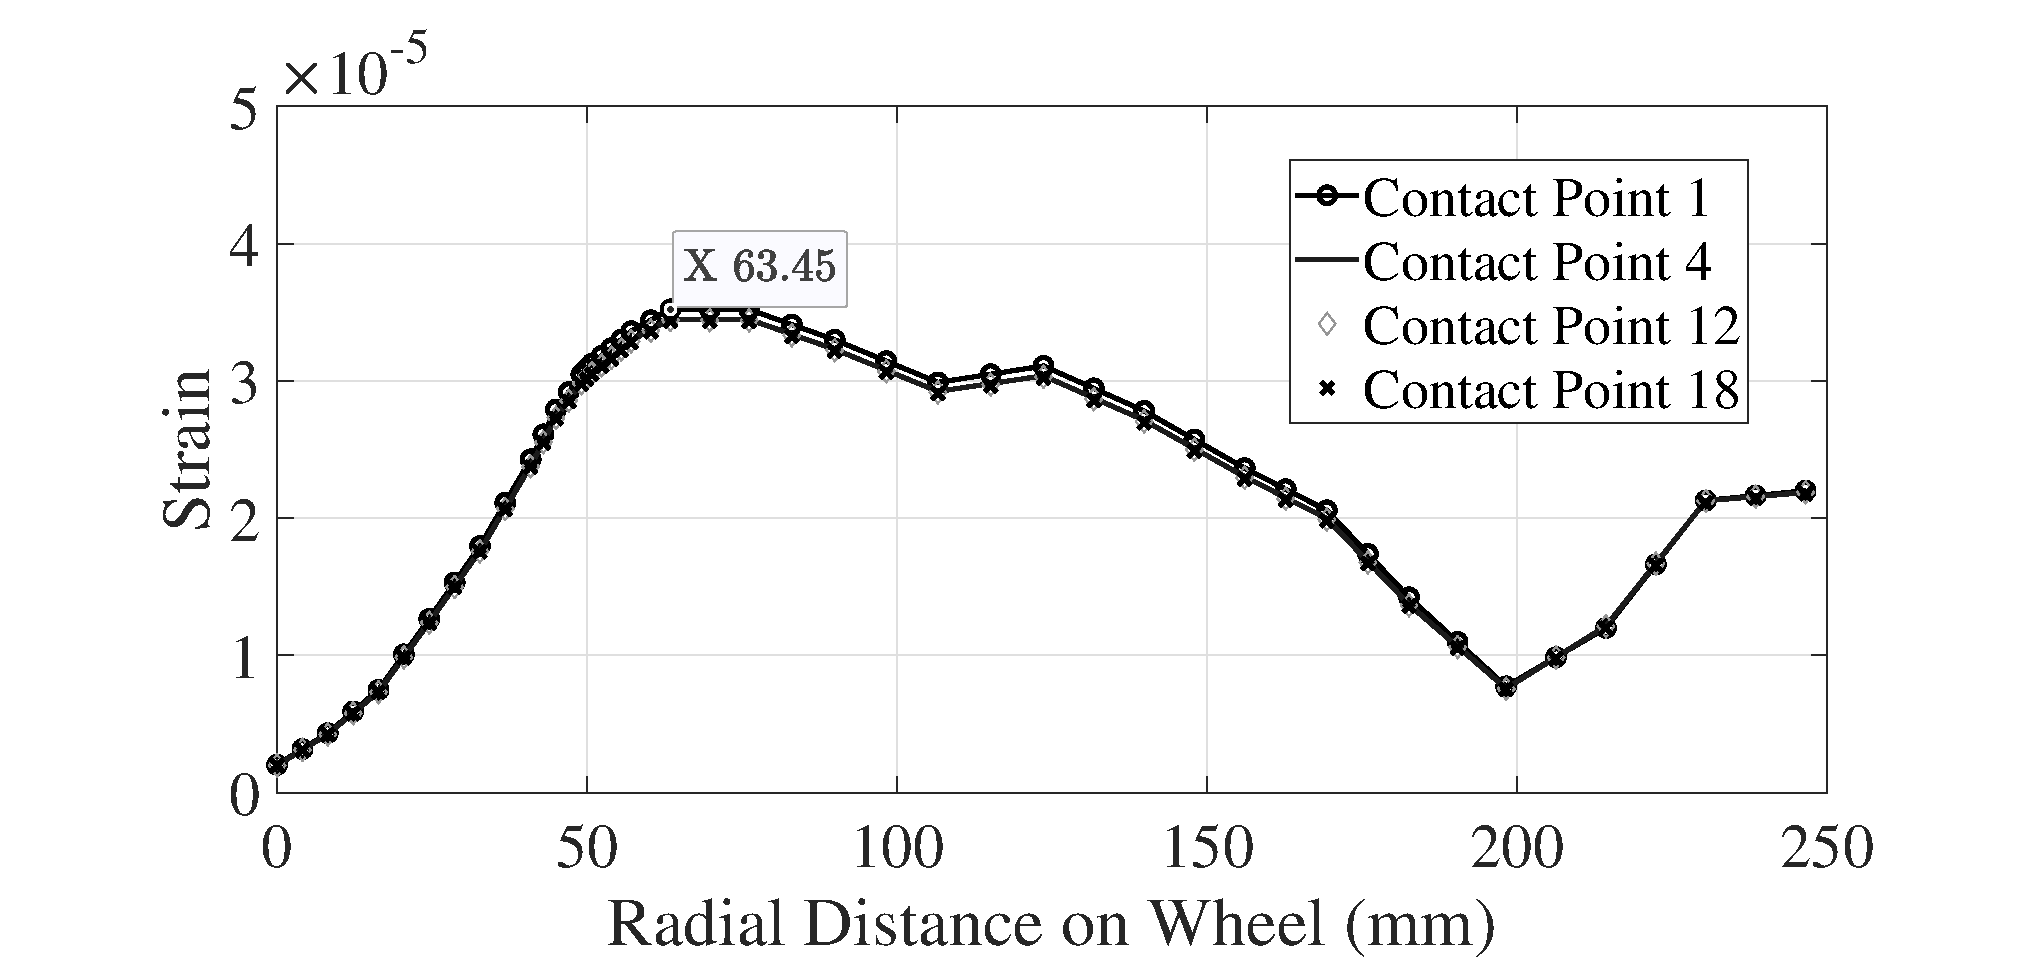
\includegraphics[width=1.0\linewidth,height=0.35\textheight]{latout.eps}}}
\caption{Strain sensitive radial location due to lateral force} \label{fig:strainvertical}
\end{figure}


\begin{figure}[h]
\centering
\resizebox*{7cm}{!}{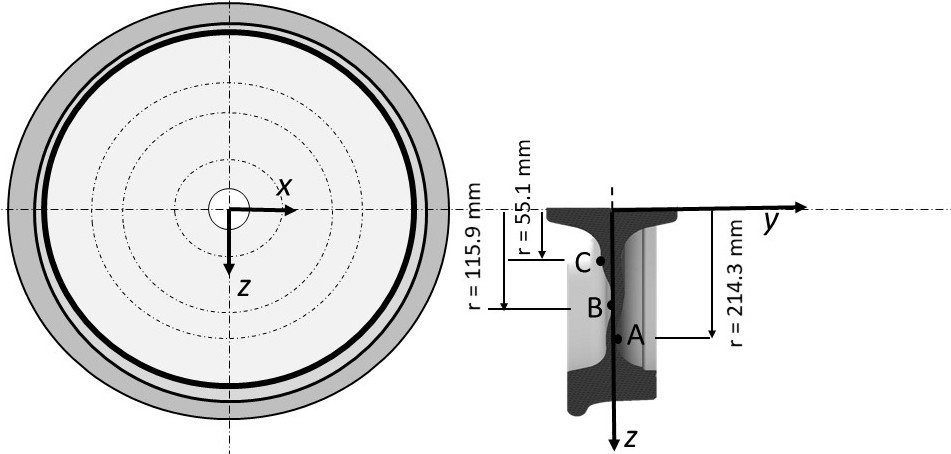
\includegraphics{Radiallocation.jpg}}
\caption{ Strain sensitive radial location on the wheel} \label{fig:Radiallocation}
\end{figure}

\subsection{Optimum number and way of connecting strain gauge in Wheatstone bridge}
Strain measured from strain gauge is a function of wheel rotational velocity ($\omega$). Strain recorded by any strain gauge is maximum when it is directly above the contact point. Any other moment than this, it does not provide an actual reading. Hence we need to place more strain gauge at a radial distance to obtain a continuous reading from strain gauges.

The intensity of the rail-wheel contact force and contact point position determines the intensity of strain recorded. Strain gauge reading for different layout is noted and analysed to define the optimal solution. Various combinations of strain gauges, 4,8,12, were placed at one radial distance. These strain gauges are connected to the Wheatstone bridge as shown in \cref{fig:Wheatstonebridge} . The signal from obtaining the Wheatstone bridge is given by \cref{eq5}. For the known value of gauge factor k and strain , the output signal obtained Wheatstone bridge is given by \cref{eq6}. 

If the multiple numbers of strain gauges are placed at one radial location. Each strain gauge measures maximum strain when the strain gauge is directly above the contact point.   Signal obtained from the strain gauge and signal obtained from the Wheatstone bridge for the combination of 4 and 8 strain gauges placed at radial location B is shown in the \cref{fig:strainWBsignal}. 

From standard \cite{UIC, EN}, for every 2 m distance travelled, rail-wheel contact force should be measured.  If the number of strain gauges placed at one radial location is increased, then the strength of the signal obtained from the Wheatstone bridge also increases shown in \cref{fig:strainWBsignal}. But it is not economically feasible to place a large number of strain gauges at one radial distance. After eight strain gauges, an increase in strength of the signal obtained from the Wheatstone bridge is minimal. Hence eight strain gauges are placed at every radial location. A total of 24 strain gauges are needed to place in each wheel.


\begin{figure}[h]
\centering

\subfloat[ Number of  strain gauges on the wheel]{%
\resizebox*{4cm}{!}{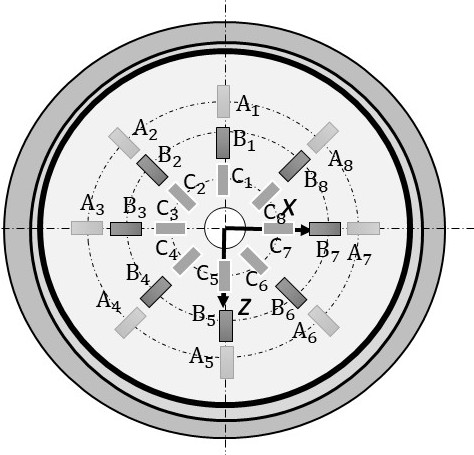
\includegraphics{Wheatstonearrangement.jpg}}}
\subfloat[Way of connecting strain gauges in  Wheatstone bridge ]{%
\resizebox*{4cm}{!}{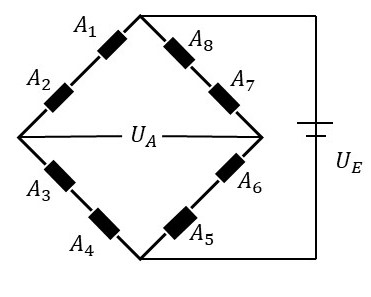
\includegraphics{Wheatstonebridge.jpg}}}


\caption{Optimal layout and number of strain gauges placed on wheel} \label{fig:Wheatstonebridge}
\end{figure}

\begin{equation}
\frac{U_A}{U_E}= \frac{\Delta R_1}{R_1} +\frac{\Delta R_2}{R_2}-\frac{\Delta R_3}{R_3}-\frac{\Delta R_4}{R_4}+\frac{\Delta R_5}{R_5} +\frac{\Delta R_6}{R_6}-\frac{\Delta R_7}{R_7}-\frac{\Delta R_8}{R_8} \label{eq5}
\end{equation}
\begin{equation}
\frac{U_A}{U_E} = \epsilon_1+\epsilon_2-\epsilon_3-\epsilon_4+\epsilon_5+\epsilon_6-\epsilon_7-\epsilon_8 \label{eq6}
\end{equation}

\begin{figure}[h]
\centering

\subfloat[ Strain variation measured from four strain gauges]{%
\resizebox*{7cm}{!}{\includegraphics{4straingauge.eps}}}
\subfloat[Strain signal measured from four strain gauges connected Wheatstone bridge ]{%
\resizebox*{7cm}{!}{\includegraphics{4straingaugesWB.eps}}}
\\
\subfloat[ Strain variation measured from eight strain gauges]{%
\resizebox*{7cm}{!}{\includegraphics{8straingauge.eps}}}
\subfloat[Strain signal measured from eight strain gauges connected Wheatstone bridge ]{%
\resizebox*{7cm}{!}{\includegraphics{8straingaugeWB.eps}}}

\caption{Signal measured from strain gauges  placed on wheel} \label{fig:strainWBsignal}
\end{figure}

\section{Formulation of Transfer Function between Input and Output}
\subsection{Develop analytical transfer function between strain as input and rail-wheel forces as output}
Strain in a wheel is a function of lateral force, vertical force, and contact point $L_V$ as given by \cref{eq4}. We have three input parameters that are needed to calculate; hence We have chosen radial three points on a wheel for strain calculation. These locations are A, B, C. \cref{eq8} shows strain relation at these locations. The relationship between strain and input parameters is linear.The relationship between strain and contact forces formulated in matrix form given by \cref{eq:Matrix}. The individual coefficient in the \cref{eq8} is calculated by varying a single parameter at a time while performing the simulation. The detail description of the various input parameter is given in the Table \ref{tab4}. The \cref{straininput}  shows the result obtained from the simulation.

Apart from contact forces, strain in the wheel also present due to axle load, wear, temperature. Initial calibration is performed on the strain by varying vertical force, as shown in \cref{calibration}, and the value of the constants $\theta_{A0}$, $\theta_{B0}$, $\theta_{C0}$ are calculated. 

\begin{equation}
\begin{aligned}
  \epsilon_A = \theta_{A0} + \theta_{A1}F +  \theta_{A2}FL_V+ \theta_{A3}Q          \\
  \epsilon_B =\theta_{B0} +  \theta_{B1}F +  \theta_{B2}FL_V+ \theta_{B3}Q  \\
\epsilon_C = \theta_{C0} + \theta_{C1}F +  \theta_{C2}FL_V+ \theta_{C3}Q 
\end{aligned}
\label{eq8}
\end{equation}

\begin{equation} \label{eq:Matrix}
\def\arraystretch{1.2}%
\begin{bmatrix}
$\epsilon_{Acalibrated}$ \\
$\epsilon_{Bcalibrated}$\\
$\epsilon_{Ccalibrated}$\\
\end{bmatrix}
=\begin{bmatrix}
\theta_{A1} & \theta_{A2}& \theta_{A3} \\
\theta_{B1} & \theta_{B2} & \theta_{B3}\\
\theta_{C1} & \theta_{C2} & \theta_{C3} \\
\end{bmatrix}
\begin{bmatrix}
F \\
FL_V\\
Q\\
\end{bmatrix}
+\begin{bmatrix} 
\theta_{A0}  \\
\theta_{B0} \\
\theta_{C0}  \\
\end{bmatrix}
\end{equation}

\begin{table}[h]
\tbl{Parameter used for numerical simulation}
{\begin{tabular}{  m{9.2em}  m{3cm} m{3cm}   m{3cm}}
\toprule
  \textbf{Case}& \textbf{1} &\textbf{2}  &\textbf{3}  \\ 
 \midrule
\textbf{Lateral force(Q)}& 20 kN & 10 kN & 7.5 -- 12.5 kN \\ 
\textbf{Vertical force(F)}& 50 -- 145 kN & 100 kN & 100 kN \\ 
\textbf{Contact point($L_V$)}& -6 mm & -6 mm -- +6 mm & -6 mm \\ 
\textbf{Remark}& Vertical force is increased in step size of 5 kN & Contact point is changed in step size of 0.5 mm & Lateral force is increased in step size of 2.5 kN \\ 
\textbf{Equation}& $\epsilon_A$ = Constant + F($\theta_{A1}$ + $\theta_{A2}$) & $\epsilon_A$ = Constant +  $\theta_{A2}$ $L_V$  & $\epsilon_A$ = Constant + $\theta_{A3}$ Q \\ 

\bottomrule
\end{tabular}}
\label{tab4}
\end{table}



\begin{figure}[h]
\centering
\subfloat[Strain vs Vertical force, case 1.]{%
\resizebox*{7cm}{!}{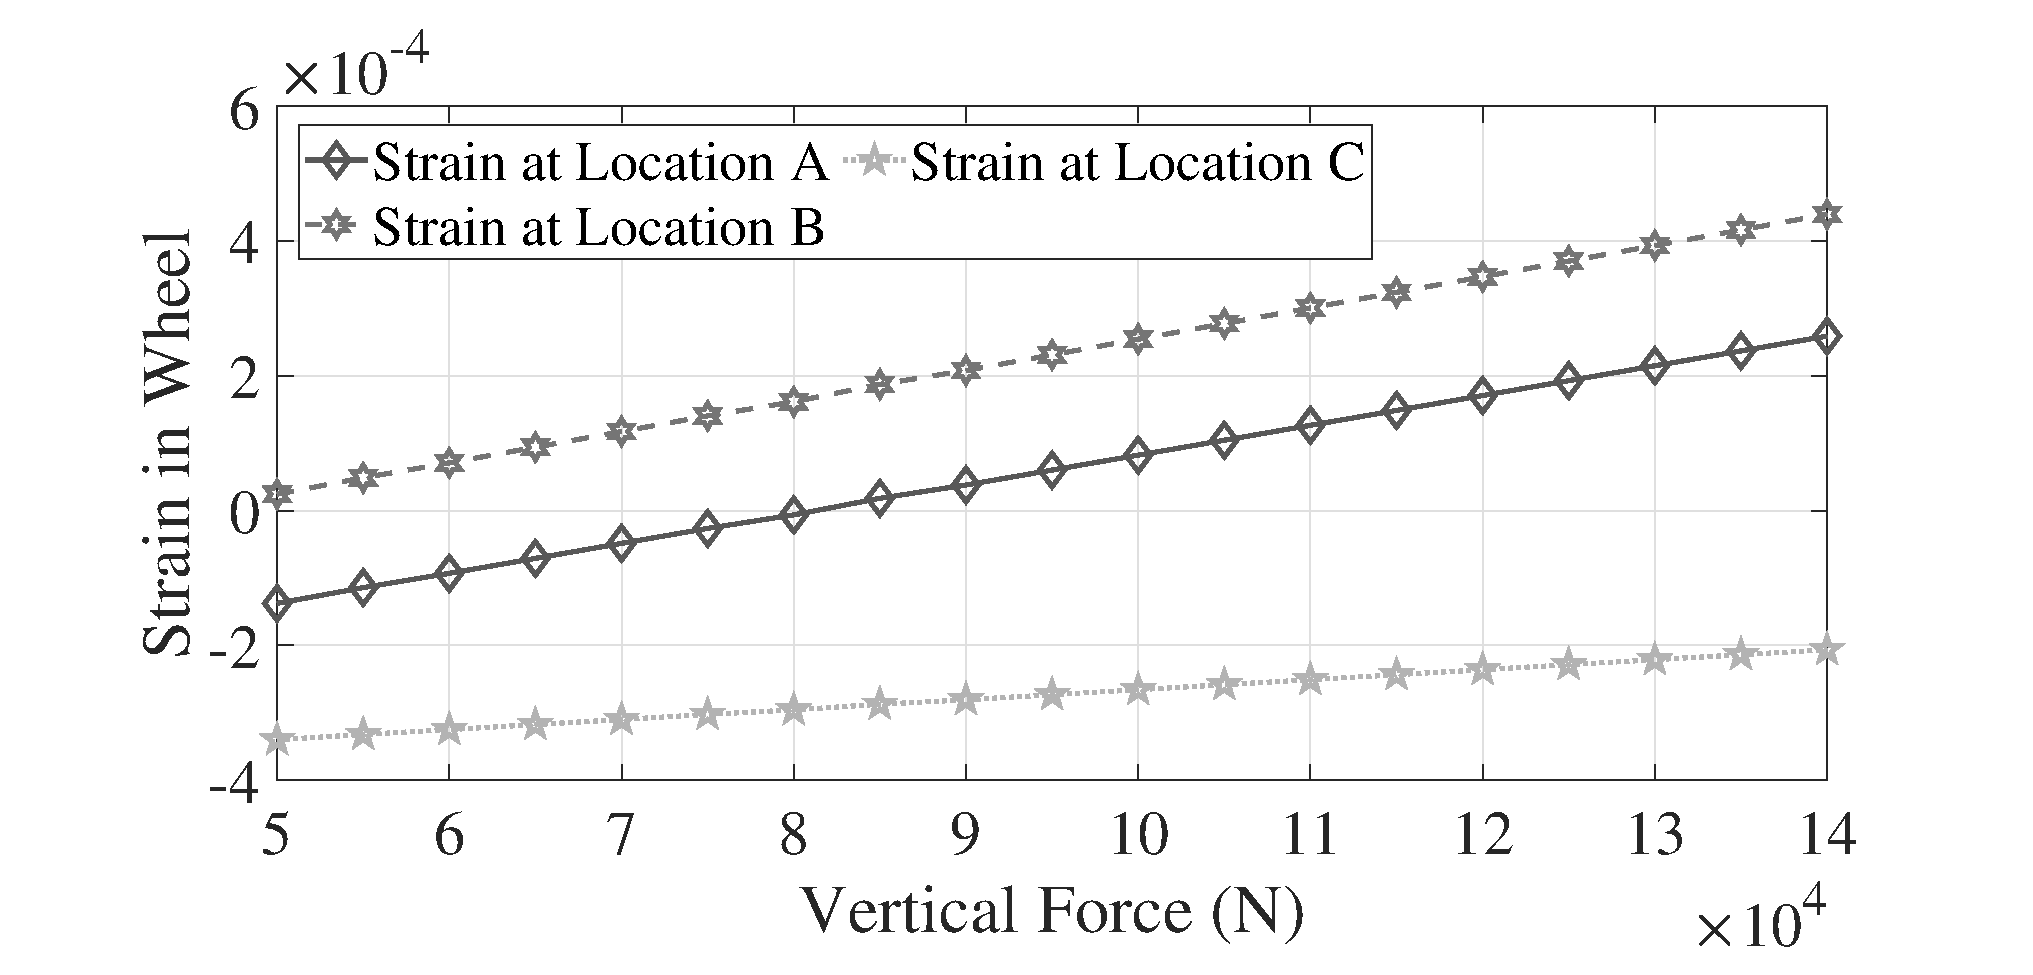
\includegraphics{verticalchange.eps}}}
\subfloat[Strain vs Lateral force, case 2.]{%
\resizebox*{7cm}{!}{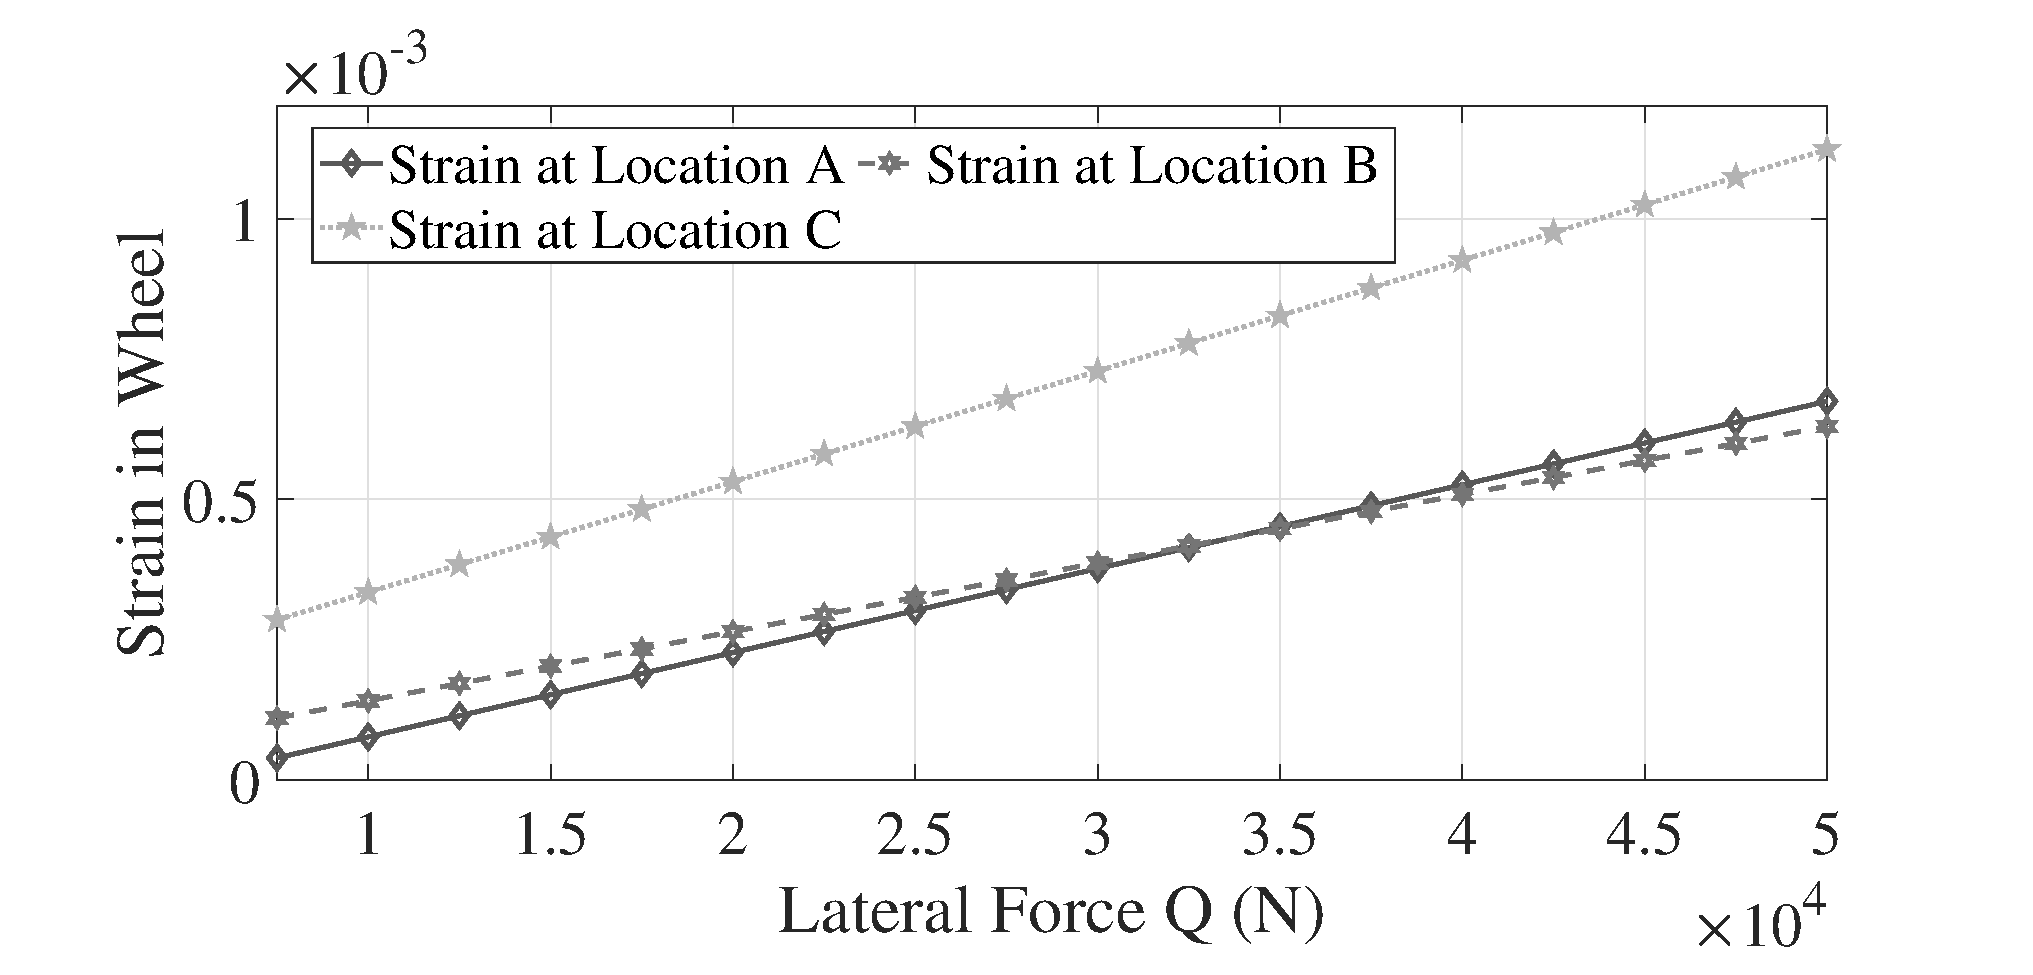
\includegraphics{Lateralchange.eps}}}

\subfloat[Strain vs contact point variation in lateral direction, case 3.  ]{%
\resizebox*{7cm}{!}{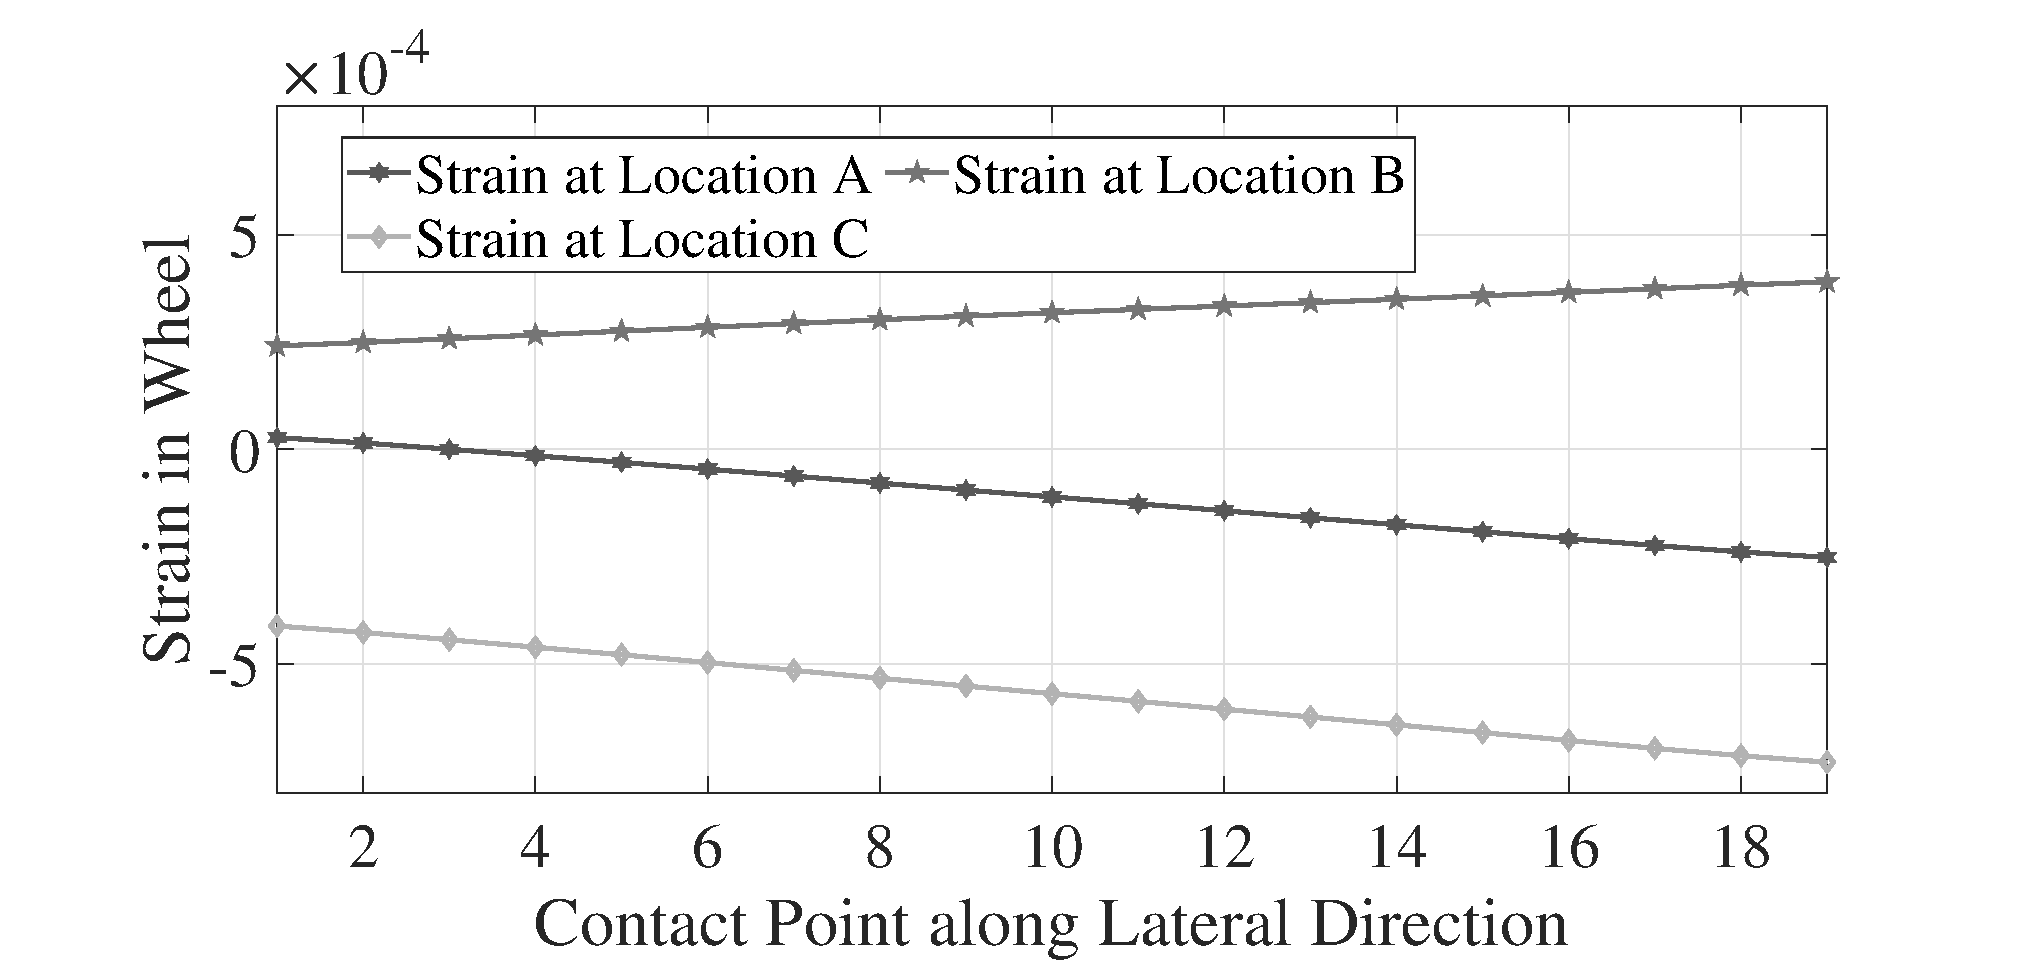
\includegraphics{contactpointchange.eps}}}

\caption{Strain vs contact input parameter variation.} \label{straininput}
\end{figure}

\begin{figure}[h]
\centering
\subfloat[ Calculation of  $\theta_{A0}$]{%
\resizebox*{7cm}{!}{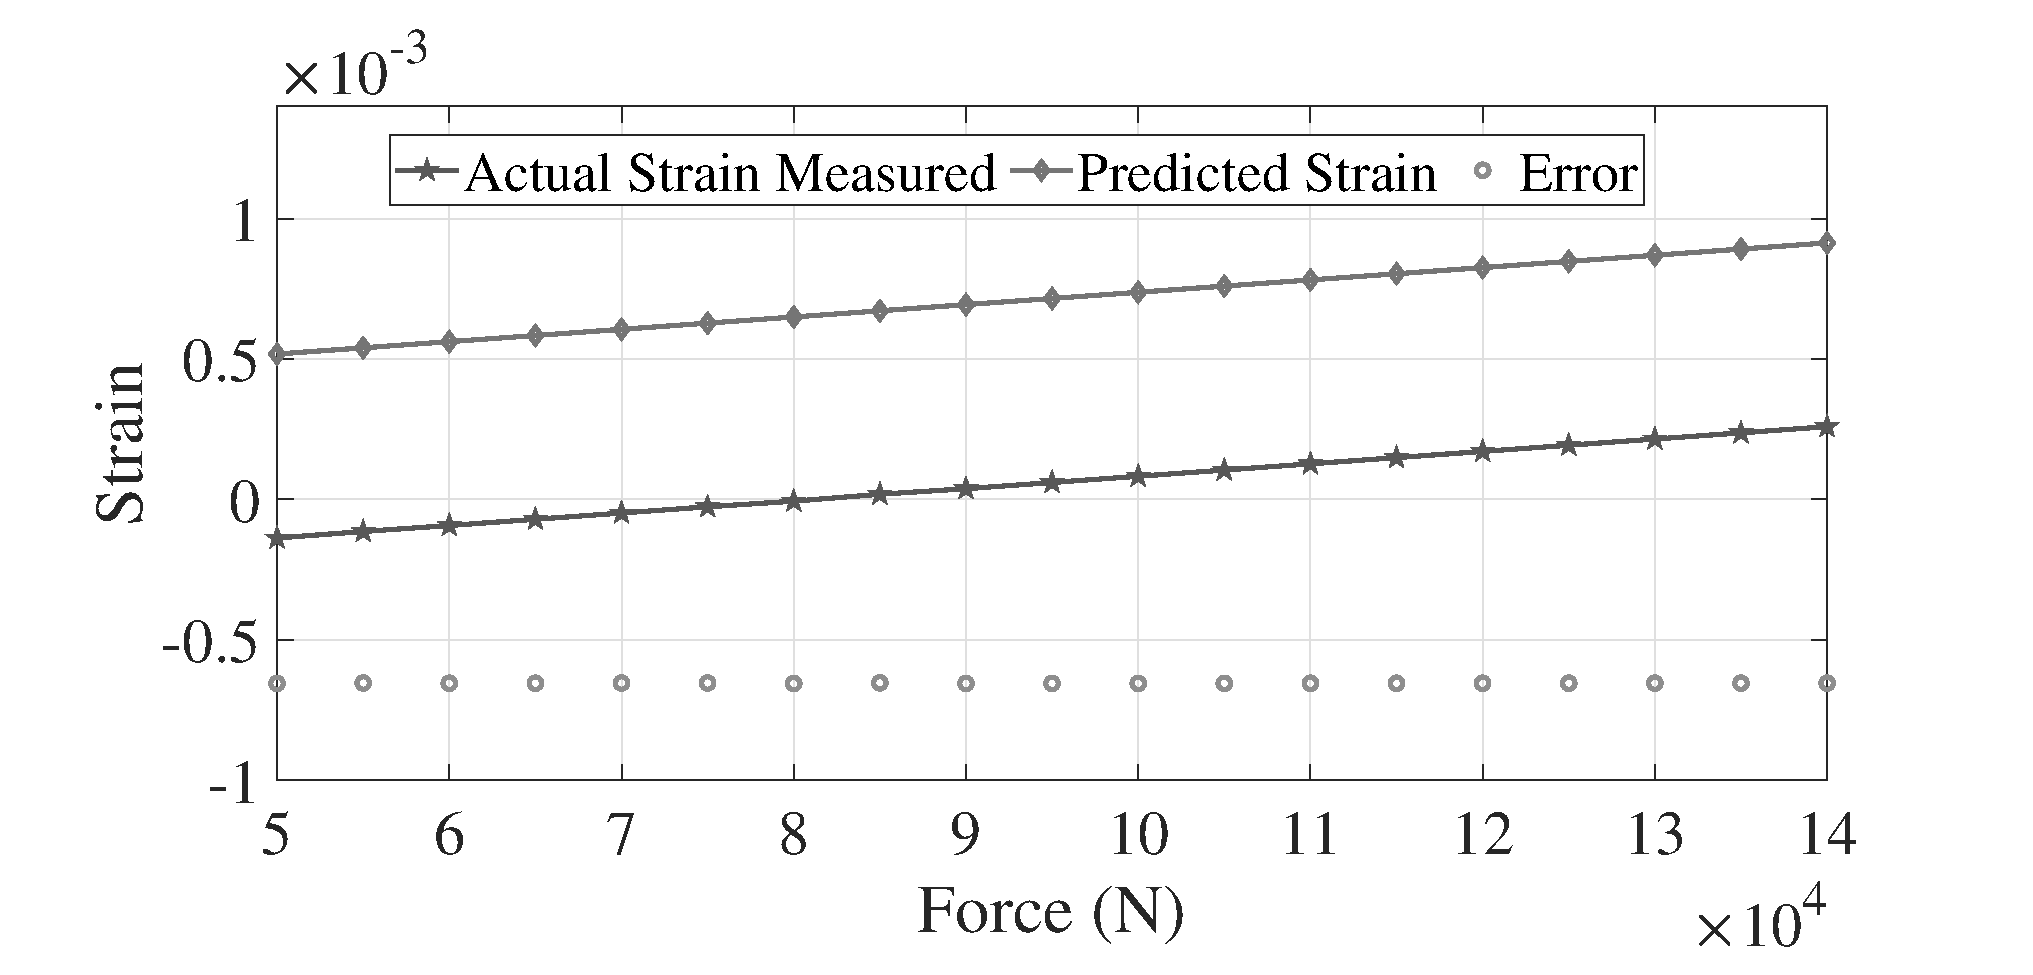
\includegraphics{ThetaA0atA.eps}}}
\subfloat[Calculation of  $\theta_{B0}$]{%
\resizebox*{7cm}{!}{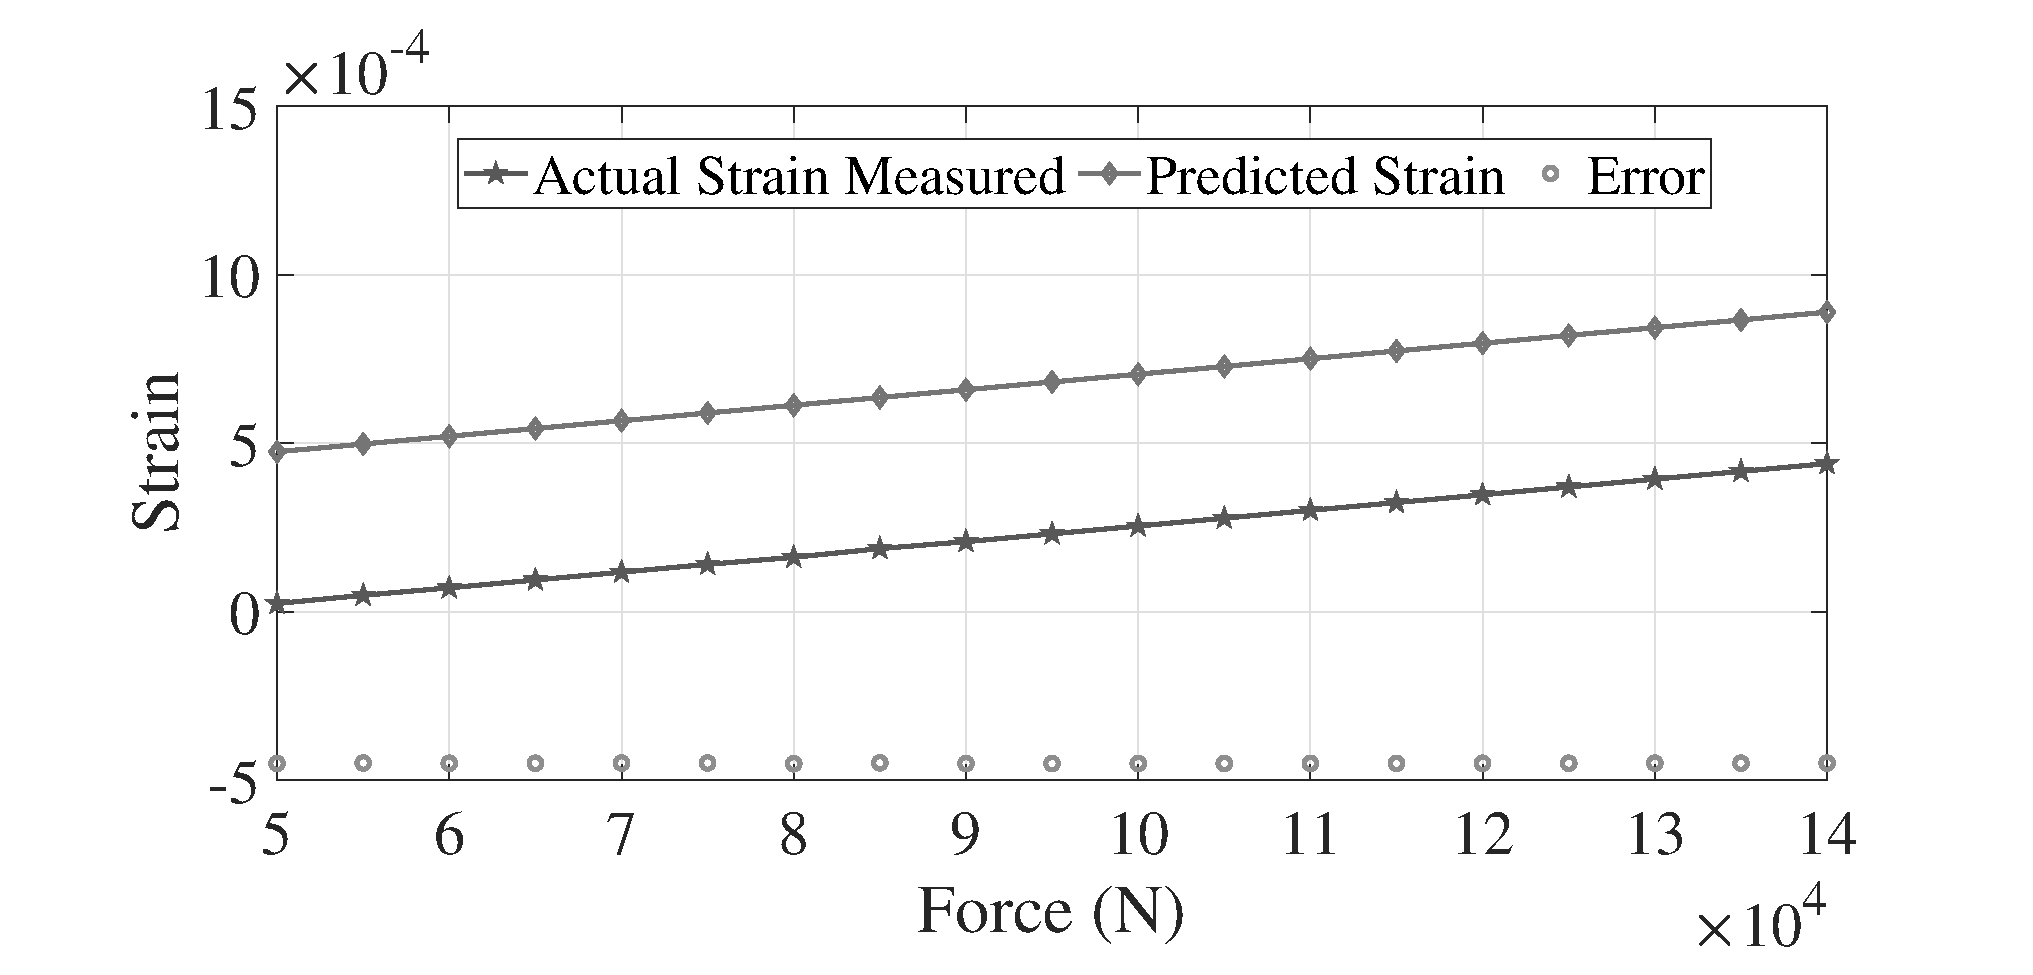
\includegraphics{ThetaB0atB.eps}}}

\subfloat[Calculation of  $\theta_{C0}$ ]{%
\resizebox*{7cm}{!}{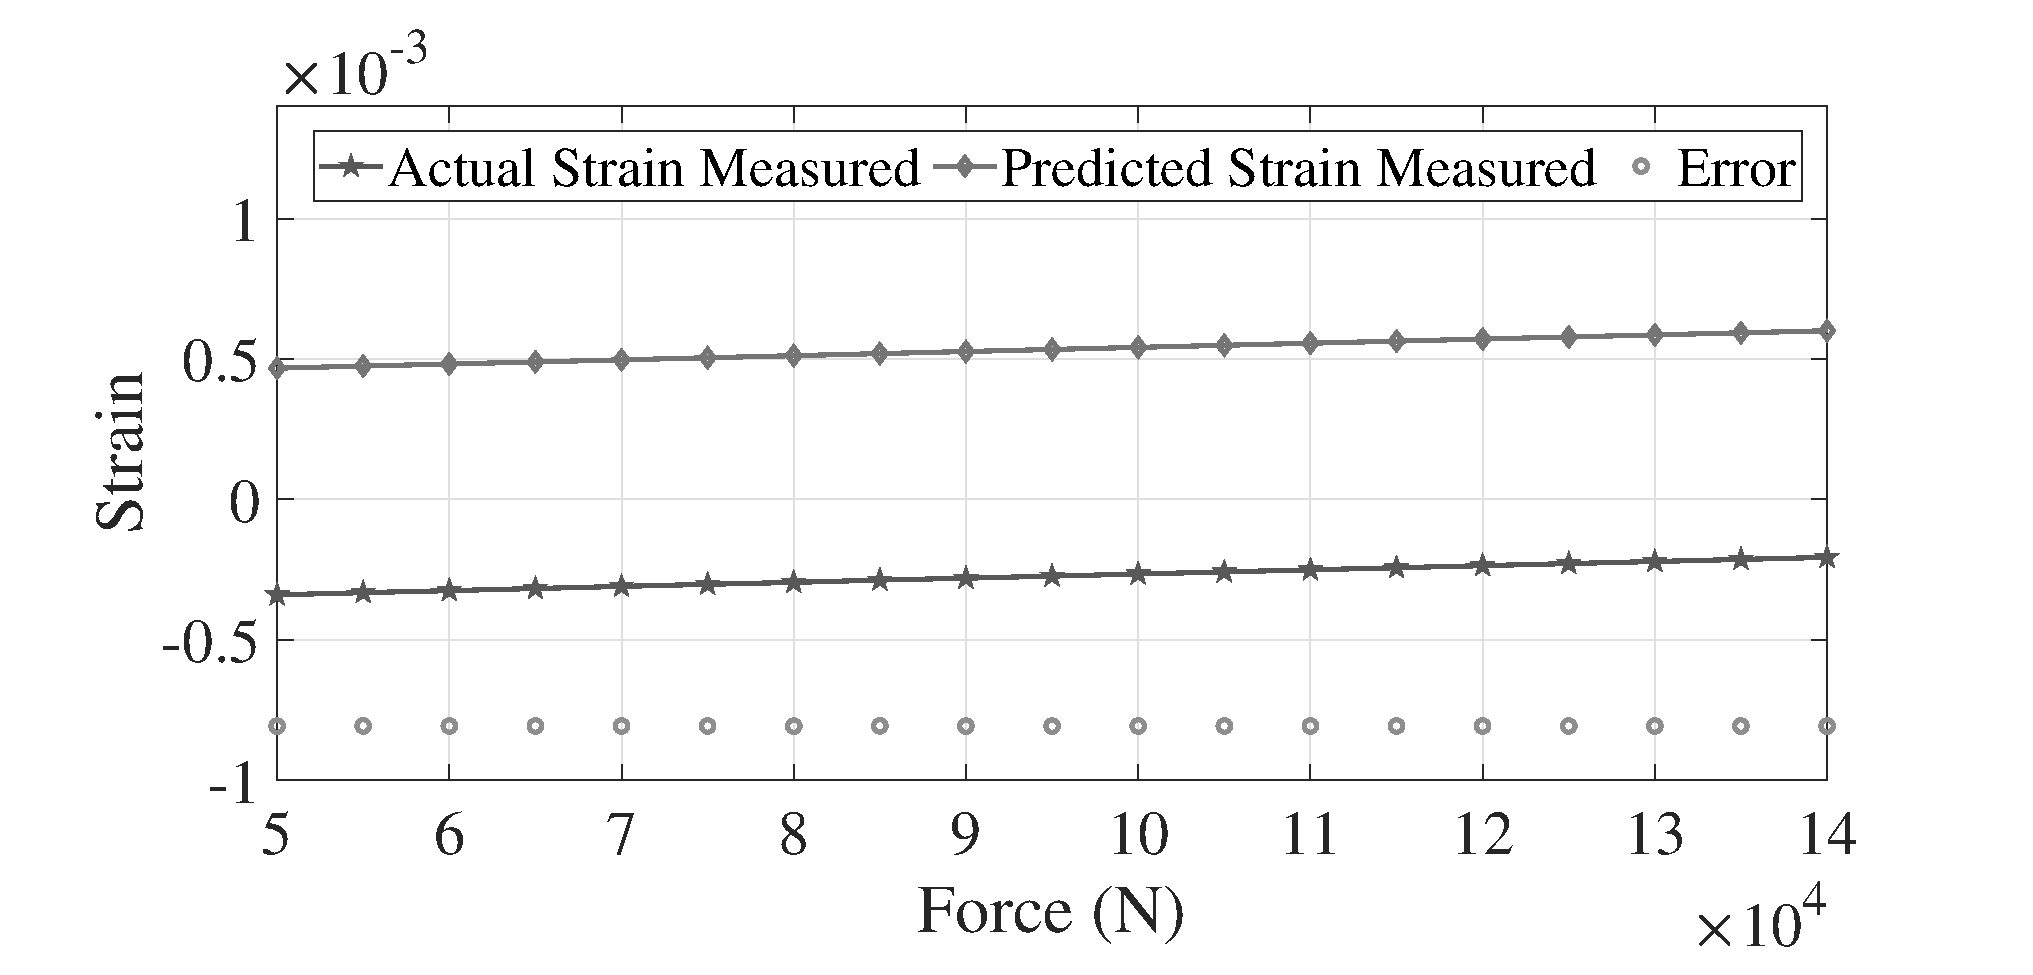
\includegraphics{ThetaC0atC.eps}}}
\caption{Initial Calibration to calculate constants.} \label{calibration}
\end{figure}



\begin{equation} \label{eq:StrainCalibration}
\def\arraystretch{1.2}%
\begin{bmatrix}
$\epsilon_{Acalibrated}$ \\
$\epsilon_{Bcalibrated}$\\
$\epsilon_{Ccalibrated}$\\
\end{bmatrix}
=\begin{bmatrix}
$\epsilon_{A}$ - $\theta_{A0}$ \\
$\epsilon_{B}$ - $\theta_{B0}$\\
$\epsilon_{C}$ - $\theta_{C0}$\\
\end{bmatrix}
=\begin{bmatrix}
$\epsilon_{A}$ - 6.54*10^{-4} \\
$\epsilon_{B}$ - 4.49*10^{-4}\\
$\epsilon_{C}$ - 8.06*10^{-4}\\
\end{bmatrix}
\end{equation}


\begin{equation} \label{eq:Relation}
\def\arraystretch{1.2}%
\begin{bmatrix}
$\epsilon_{Acalibrated}$ \\
$\epsilon_{Bcalibrated}$\\
$\epsilon_{Ccalibrated}$\\
\end{bmatrix}
=
10^{-9}\begin{bmatrix} 
3.04 & 0.15& 14.89 \\
5.30 & -0.8285 & 12.22\\
-0.04 & 0.17 & 19.66 \\
\end{bmatrix}
\begin{bmatrix}
F \\
FL_V\\
Q\\
\end{bmatrix}
\end{equation}

The relationship between contact forces as output and strain as the input will be obtained by taking the inverse of  \cref{eq:Relation} and is given by  \cref{eq:Inverse}.


\begin{equation} \label{eq:Inverse}
\def\arraystretch{1.2}%
\begin{bmatrix}
F \\
FL_V\\
Q\\
\end{bmatrix}
=
10^{9}\begin{bmatrix} 
0.26 & 0.031& -0.22 \\
7.39 & -4.27 & -2.95\\
-0.06 & 0.03 & 0.77 \\
\end{bmatrix}
\begin{bmatrix}
\epsilon_{Acalibrated} \\
\epsilon_{Bcalibrated}\\
\epsilon_{Ccalibrated}\\
\end{bmatrix}
\end{equation}

\section{Validation}
Numerical simulation is performed to demonstrate the effectiveness of the developed method. Vertical force is varied from 50 kN to 85 kN, and lateral force varied from 25 kN to 60 kN. The contact point is changed laterally while performing simulation to validate the formulated relationship. The absolute error of measurement of the parameter F, Q, L, Q/F ratio is shown in the \cref{validation}. Mean absolute error and percentage error while measurement of parameters is given in Table \ref{tab5}.  

\begin{table}[h]
\tbl{Error involved in measurement of parameters}
{\begin{tabular}{  m{10em}  m{8em} m{8em}} 
\toprule
  \textbf{Parameters}& \textbf{Mean absolute error}  & \textbf{Percentage error}\\ 
 \midrule
\Vertical force (F)& 171.21 & 0.215\\ 
Lateral force (Q)&  25.92 & 0.049\\ 
Contact point ($L_V$)&  0.65 & 3.62 \\ 
Q/F ratio &  0.0013  &  0.19 \\ 

\bottomrule
\end{tabular}}
\label{tab5}
\end{table}




\begin{figure}[h]
\centering
\subfloat[  Vertical force (F) estimation ]{%
\resizebox*{7cm}{!}{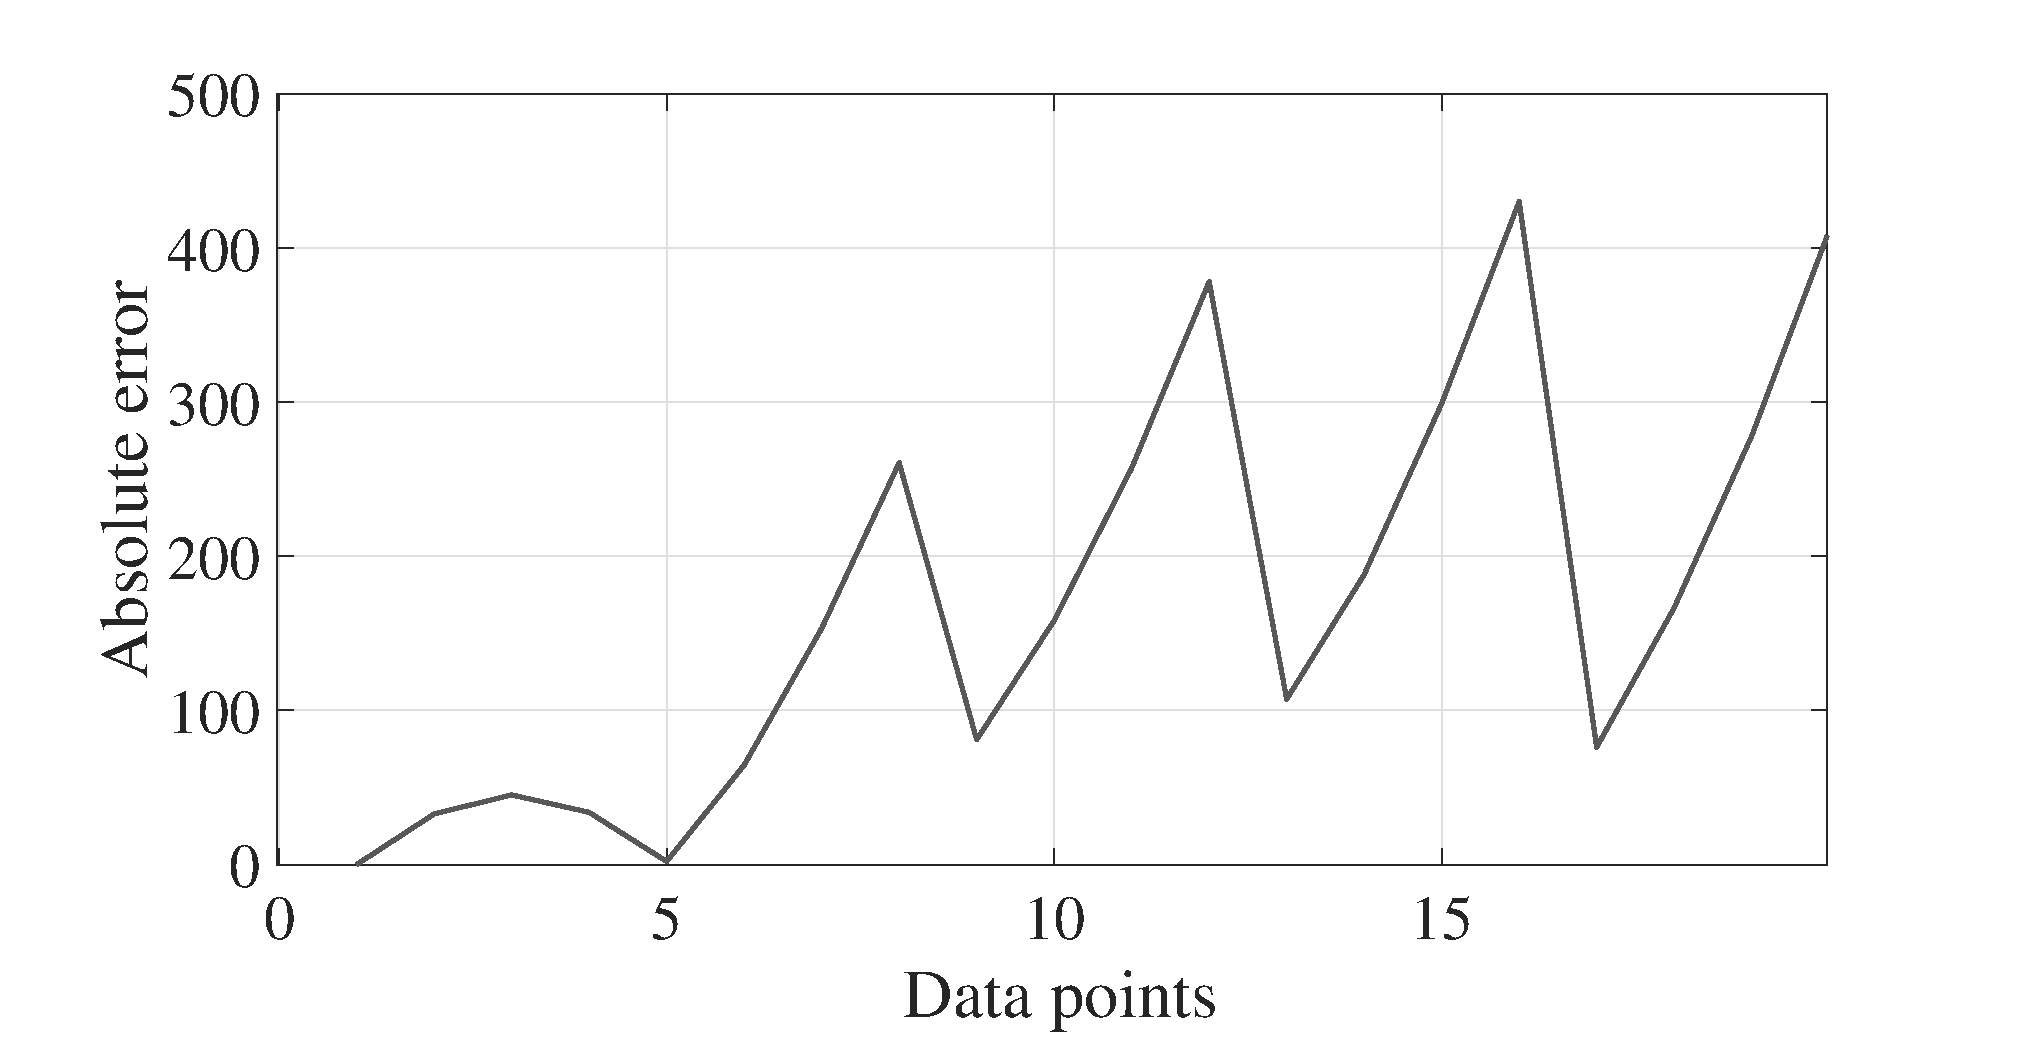
\includegraphics{vertical.eps}}}
\subfloat[Lateral force (Q) estimation]{%
\resizebox*{7cm}{!}{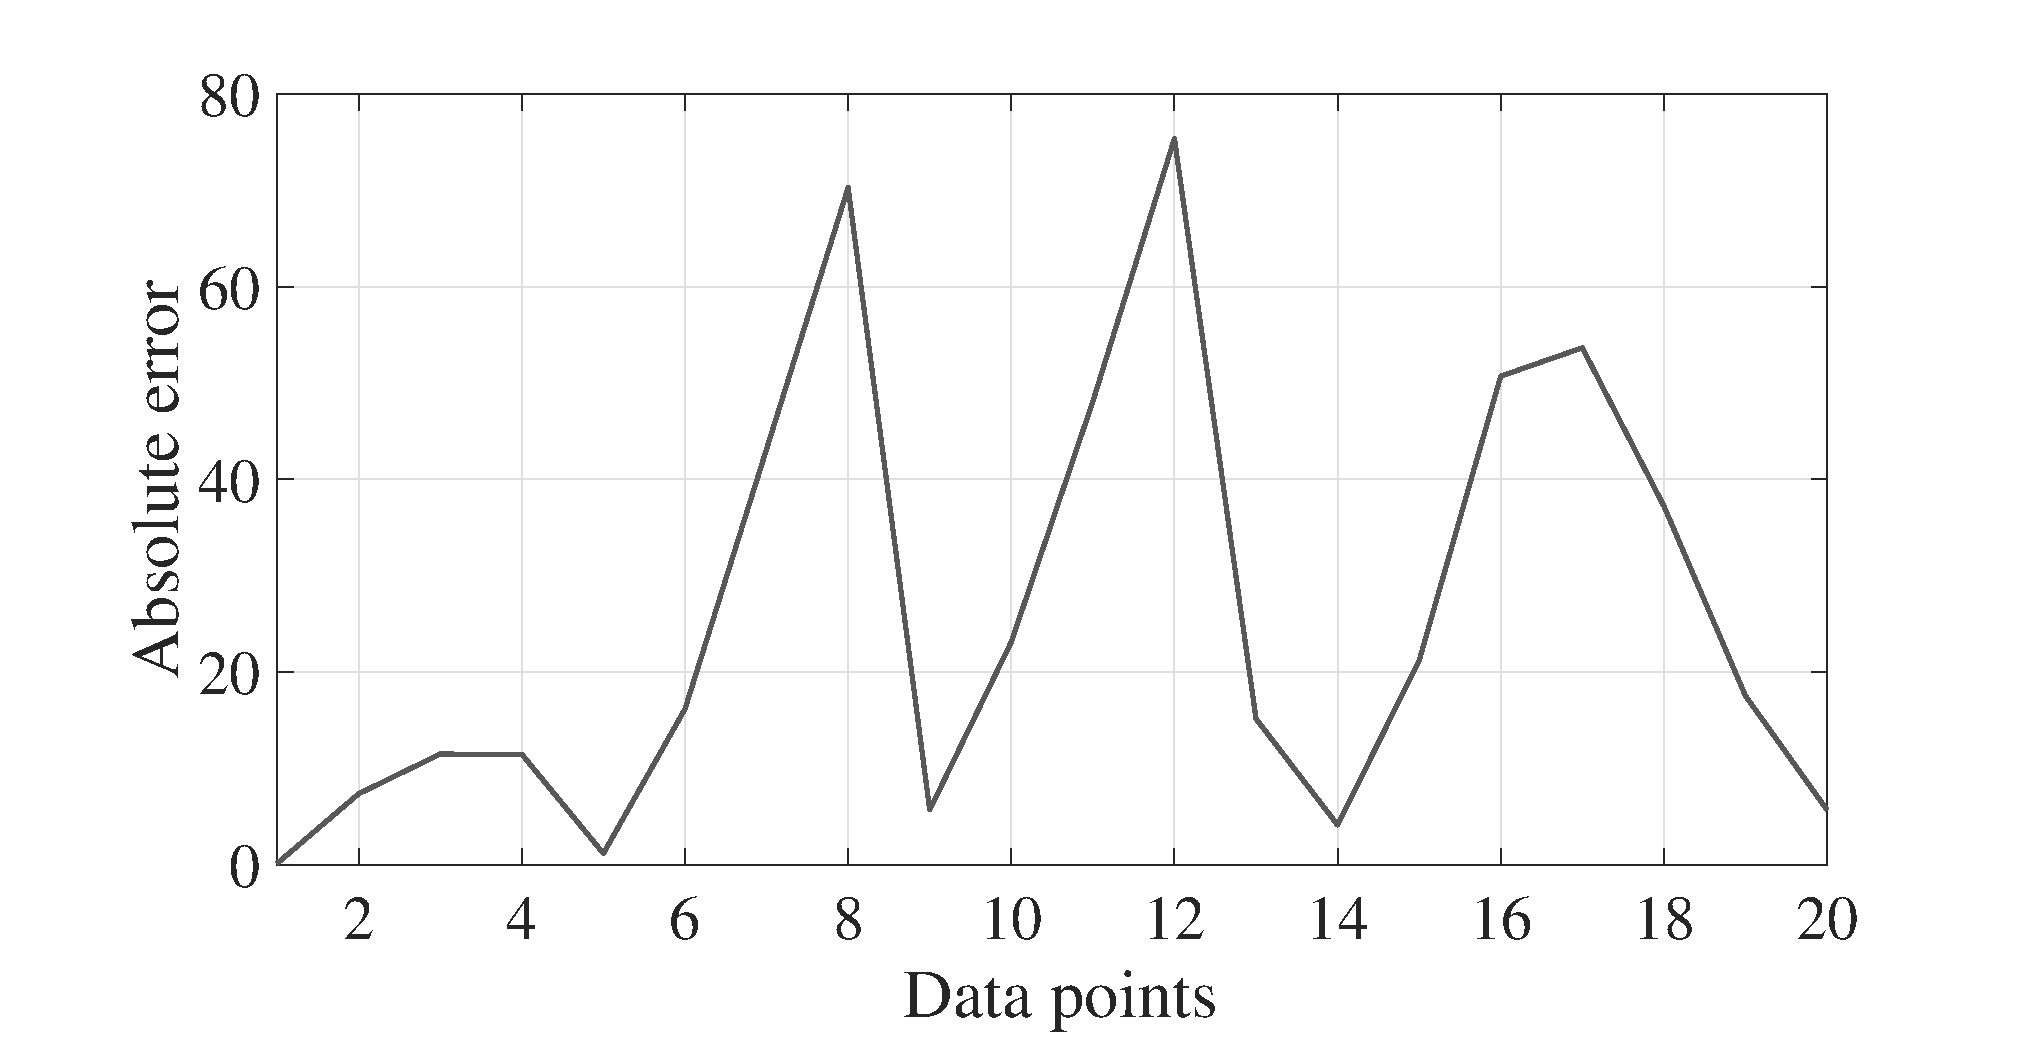
\includegraphics{lateral.eps}}}

\subfloat[Contact point($L_V$) estimation ]{%
\resizebox*{7cm}{!}{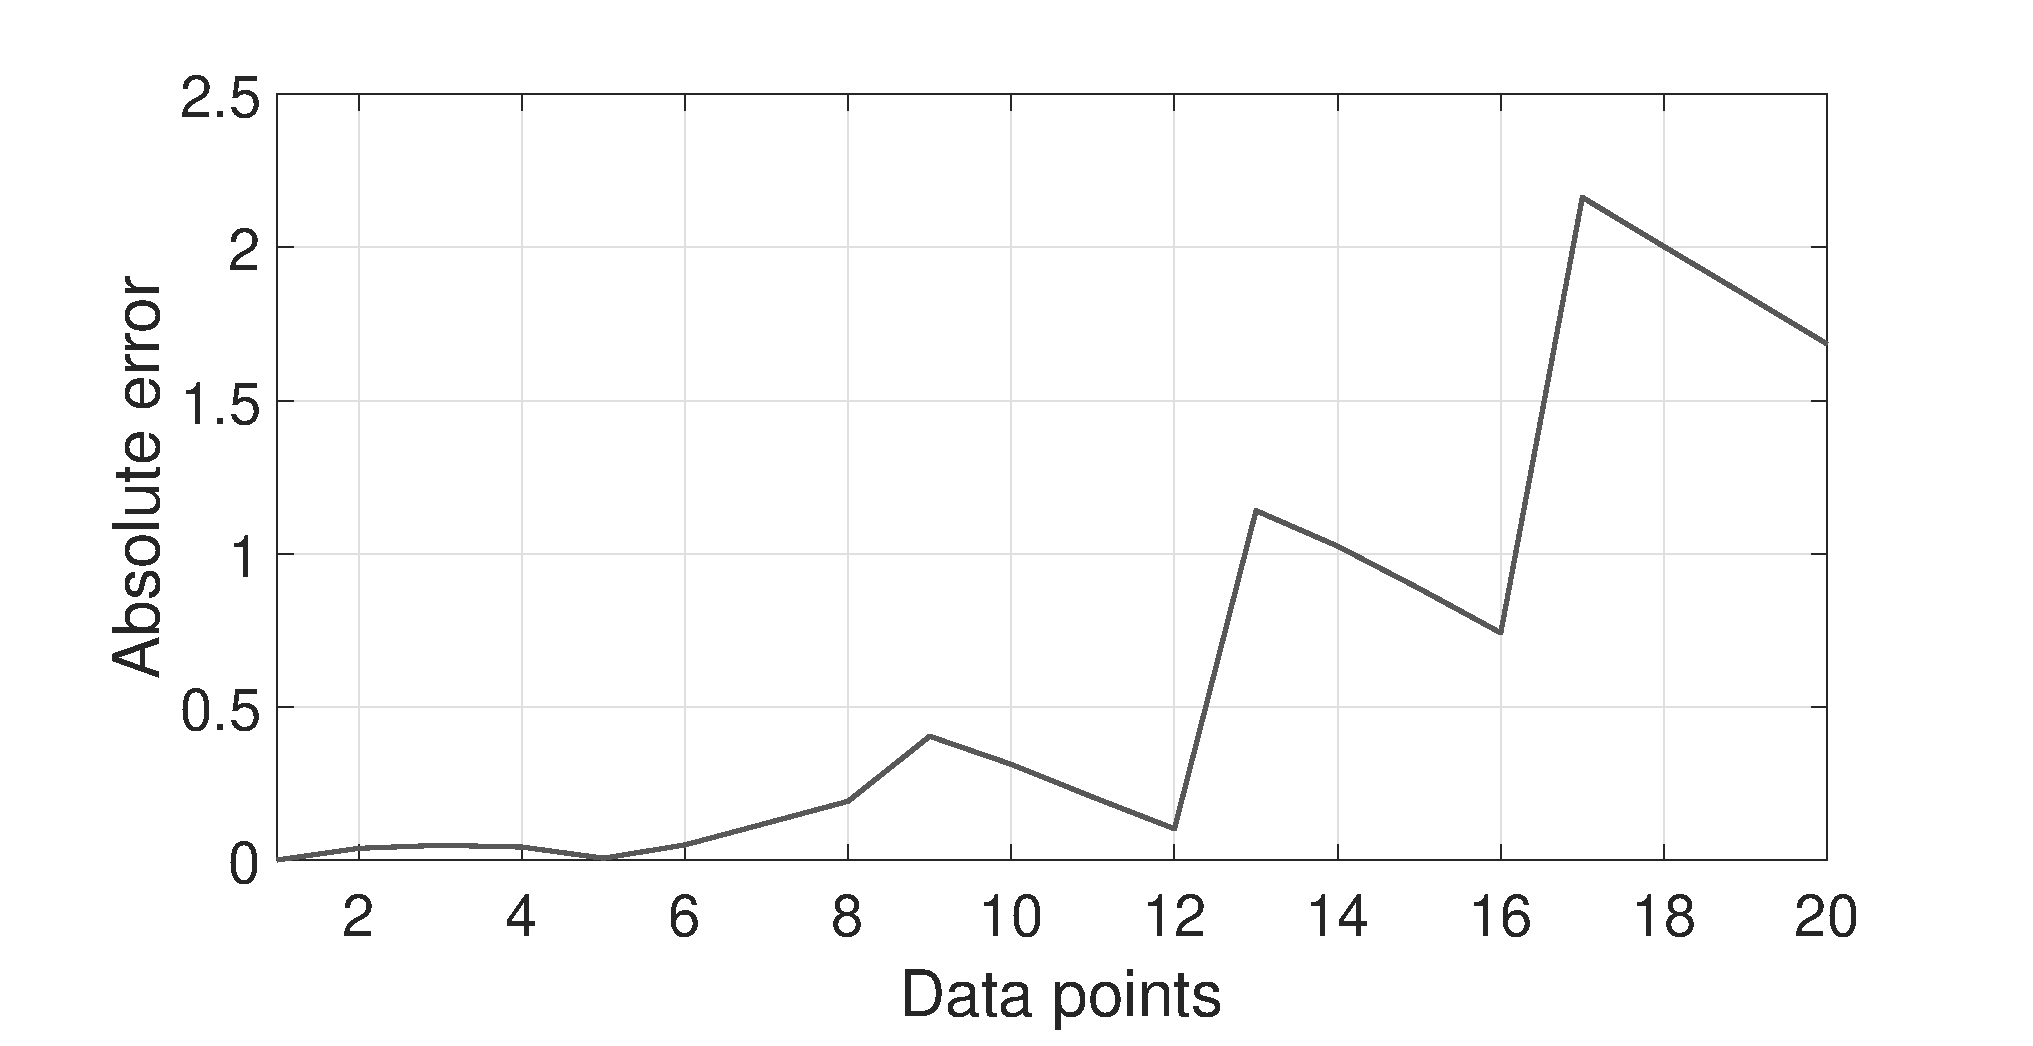
\includegraphics{contact.eps}}}
\subfloat[ Q/Fratio estimation ]{%
\resizebox*{7cm}{!}{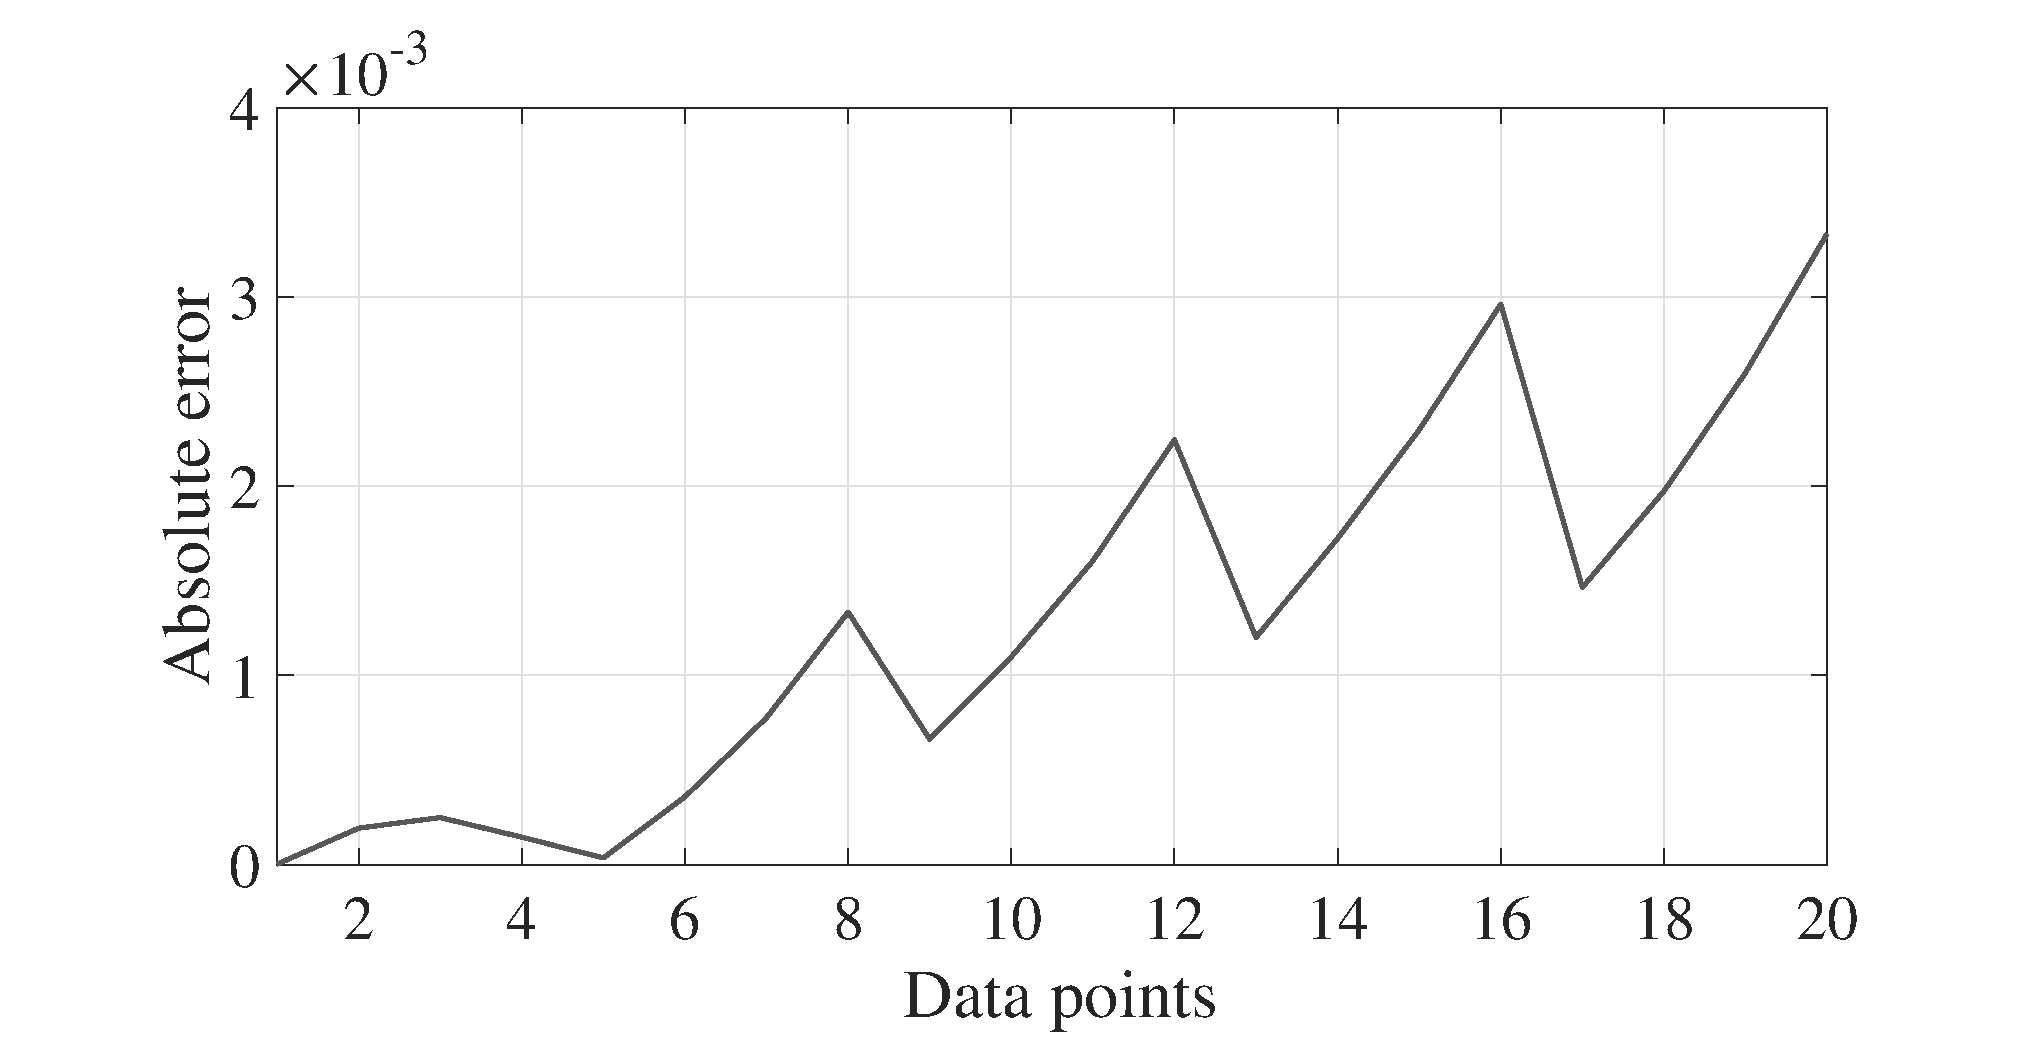
\includegraphics{Ratio.eps}}}
\caption{Absolute error associated with measurement.} \label{validation}
\end{figure}


\section{Conclusion}
The methodology of the design of measuring wheel-set using instrumenting the wheel-set by strain gauges is discussed in this study.  The relationship between strain in the wheel with contact forces and the contact point is formulated.  The radial strain sensitivity of the rail-wheel under the effect of individual parameters is discussed. Three radial location r = 55.19 mm and r = 155.9 at the inner side of the wheel and r = 214.3 mm at the outer side of the wheel is choose to place the strain gauge on the wheel. Eight strain gauges are placed on the wheel at each radial location and connected in Wheatstone bridge. The relationship between strain in a wheel with individual parameters is formulated at these three radial locations.  Numerical simulation is performed to validate the formulated relationship. The percentage error involved in calculating the contact force is less than 1 \%, and the Percentage error involved in predicting the contact point location is less than 4 \%. 









\begin{thebibliography}{}
\bibitem{Pater1}
A.D. De Pater., “The equation of motion of a single wheelset moving along a perfect track,” Veh. Syst. Dyn.1988; vol. 17, no. sup1, pp. 287–299.

\bibitem{Pater2}
A.D. De Pater., “The Geometrical Contact brtween Track and Wheelset,” Veh. Syst. Dyn. 1988, vol. 17, pp. 127–140.

\bibitem{Hertz}
H. J., “Maths,” Crelle’s, 1881.

\bibitem{Carter}
F. W. Carter, “The electric locomotive,” proc. Inst. Civ. Engs.221. p, no. 221–252.


\bibitem{Kalker1}
. J. Kalker, “The tangential force transmittted by two elaastic bodies rolling over each other with pure creepage,” Wear, vol. 11, pp. 421–430, 1968.

\bibitem{Kalker2}
J. J. Kalker, “A strip theory for rolling with slip and spin,” Proc. Kon. Ned. Akad. van Wetenachappen, Amsterdam, vol. B70, pp. 10–62, 1966.

\bibitem{Kalker3}
J. J. Kalker, “On the rolling contact of two elastic bodies in the presence of dry friction,” PhD Thesis, DELFT, 1967.

\bibitem{Kalker4}
J. J. Kalker, “Three Dimensional Elastic Bodies in Rolling Contact,” 1990.

\bibitem{Kalker5}
J. J. Kalker, “A fast algorithm for the simplified theory of rolling contact,” Veh. Syst. Dyn. 11, pp. 1–13, 1982.

\bibitem{Mil13}
Milkovic D, Simic G, Jakovljevic Z, Tanaskovic J, Lucanin V. Wayside system for wheel–rail contact forces measurements. Measurement. 2013;46(9):3308-3318.

\bibitem{Matsumoto}
A. Matsumoto et al., “Continuous observation of wheel/rail contact forces in curved track and theoretical considerations,” Veh. Syst. Dyn., vol. 50, no. SUPPL. 1, pp. 349–364, 2012, doi: 10.1080/00423114.2012.669130.

\bibitem{ORE}
ORE B55/RP4 1970 Two axled wagons subjected to simultaneous stresses due to track distortion and to transverse components of the forces of the automatic coupler Dynamic Effects of Track Distortions (Utrecht: Office de Recherches et d’Essais)

\bibitem{Fxia}
Xia F, Cole C, Wolfs P. Grey box-based inverse wagon model to predict wheel–rail contact forces from measured wagon body responses. Vehicle System Dynamics. 2008;46 Suppl 1:469-79.

\bibitem{Fxia1}
Xia F, Cole C, Wolfs P. An inverse railway wagon model and its applications. Vehicle system dynamics. 2007;45(6):583-605.

\bibitem{Chris}
Ward CP, Goodall RM, Dixon R. Contact force estimation in the railway vehicle wheel-rail interface. IFAC Proceedings Volumes. 2011;44(1):4398-4403.

\bibitem{Ward}
Ward CP, Goodall RM, Dixon R, Charles GA. Adhesion estimation at the wheel–rail interface using advanced model-based filtering. Vehicle System Dynamics. 2012;50(12):1797-1816.

\bibitem{Lic}
Li C, Luo S, Cole C, Spiryagin M. An overview: modern techniques for railway vehicle on-board health monitoring systems. Vehicle system dynamics. 2017;55(7):1045-70.

\bibitem{Xincan}
Xincan Jin,  "Evaluation and analysis approach of wheel–rail contact force measurements through a high-speed instrumented wheelset and related considerations", Vehicle System Dynamics, 58:8, 1189-1211, DOI: 10.1080/00423114.2019.1612073., 2020

\bibitem{Yu}
Yu Ren & Jianzheng Chen, " A new method for wheel–rail contact force continuous measurement using instrumented wheelset", Vehicle System Dynamics, 57:2, 269-285, DOI: 10.1080/00423114.2018.1460853., 2019

\bibitem{Milan}
M. B. Bižić, D. Z. Petrović, M. C. Tomić, and Z. V. Djinović, “Development of method for experimental determination of wheel-rail contact forces and contact point position by using instrumented wheelset,” Meas. Sci. Technol., vol. 28, no. 7, 2017, doi: 10.1088/1361-6501/aa666f.


\bibitem{Bagheri}
Bagheri, V.R., Tehrani, P.H. & Younesian, D. Optimal strain gauge placement in instrumented wheel-set for measuring wheel-rail contact forces. Int. J. Precis. Eng. Manuf. 18, 1519–1527 (2017). 


\bibitem{Zeng}
Zeng, J., Wei, L. & Wu, P. Safety evaluation for railway vehicles using an improved indirect measurement method of wheel–rail forces. J. Mod. Transport. 24, 114–123 (2016). https://doi.org/10.1007/s40534-016-0107-5.

\bibitem{UIC}
UIC Code 518. Testing and approval of railway vehicles from the point of view of their dynamic
behavior–safety–track fatigue–ride quality. 2nd ed. Paris: International Union of Railways;
2003

\bibitem{EN}
EN 14363. Railway Applications—Testing for the Acceptance of Running Characteristics of Railway Vehicles—Testing of Running Behavior and Stationary Tests (Brussels: European Committee for Standardization, CEN); 2005.


\bibitem{wickens}
Wickens AH. Fundamentals of rail vehicle dynamics. 1st ed. London: CRC Press; 2003.

\bibitem{Iwnicki}
Iwnicki S D Handbook of Railway Vehicle Dynamics Boca Raton, FL: CRC Press; 2006.

\bibitem{Shabana}
A. A. Shabana, M. Berzeri, and J. R. Sany, “Numerical Procedure for the Simulation of Wheel/Rail Contact Dynamics,” Dyn. Syst. Meas. Control, vol. 123, no. 2, p. 168, 2001.


\end{thebibliography}


\end{document}
